% Copyright (C) 2024 - Joseph Muré

\documentclass{beamer}

%\setbeameroption{hide notes}
%\setbeameroption{show notes}
%\setbeameroption{show only notes}

% Copyright (C) 2012 - EDF R&D - Michael Baudin

% To highlight source code
\usepackage{listings}
\definecolor{darkgreen}{rgb}{0,0.5,0}
\definecolor{violet}{rgb}{0.5,0,1}

\usepackage{lmodern}% http://ctan.org/pkg/lm

\usetheme{Montpellier}
\setbeamertemplate{navigation symbols}{} % Remove navigation
\useoutertheme{infolines}

\usepackage[utf8]{inputenc}
\usepackage[T1]{fontenc}

\usepackage{graphicx}
\unitlength=1cm
\graphicspath{{./figures/}}

\usepackage{hyperref}
\hypersetup{colorlinks=true, linkcolor=blue, linktocpage, urlcolor=blue}

\def\bx{{\bf x}}
\def\RR{\mathbb{R}}

\newcommand{\pyvar}[1]{\texttt{#1}}

\def \ot {OpenTURNS}

\definecolor{codegreen}{rgb}{0,0.6,0}
\definecolor{codegray}{rgb}{0.5,0.5,0.5}
\definecolor{codepurple}{rgb}{0.58,0,0.82}
\definecolor{backcolour}{rgb}{0.95,0.95,0.92}
\lstdefinestyle{mystyle}{
  backgroundcolor=\color{backcolour},   commentstyle=\color{codegreen},
  keywordstyle=\color{magenta},
  numberstyle=\tiny\color{codegray},
  stringstyle=\color{codepurple},
  basicstyle=\ttfamily\tiny,
  breakatwhitespace=false,         
  breaklines=true,                 
  captionpos=b,                    
  keepspaces=true,                 
  numbers=left,                    
  numbersep=5pt,                  
  showspaces=false,                
  showstringspaces=false,
  showtabs=false,                  
  tabsize=1,
  numbers=none
}

\lstset{style=mystyle, language=python}


\usepackage[
backend=biber,
style=alphabetic,
sorting=ynt
]{biblatex}

\usepackage{tikz}
\usetikzlibrary{positioning}

\renewcommand{\footnotesize}{\tiny}

%\addbibresource{something.bib}

\title[OpenTURNS]{Overview of OpenTURNS and its graphical user interface Persalys}

\author[Mur\'e et al.]{
J. Mur\'e \inst{1} \and
M. Baudin \inst{1} \and
J. Pelamatti \inst{1} \and  \\
J. Schueller \inst{2} \and
A. Marion \inst{2}
}

\institute[EDF-Phim\'eca]{
\inst{1} EDF R\&D. 6, quai Watier, 78401, Chatou Cedex - France, joseph.mure@edf.fr \and %
\inst{2} Phimeca Engineering. 18/20 boulevard de Reuilly, 75012 Paris - France, schueller@phimeca.com
}


\date[]{May 22nd 2024, BEPU 2024, Lucca, Italy}

\definecolor{codegreen}{rgb}{0,0.6,0}
\definecolor{codegray}{rgb}{0.5,0.5,0.5}
\definecolor{codepurple}{rgb}{0.58,0,0.82}
\definecolor{backcolour}{rgb}{0.95,0.95,0.92}
\lstdefinestyle{mystyle}{
  backgroundcolor=\color{backcolour},   commentstyle=\color{codegreen},
  keywordstyle=\color{magenta},
  numberstyle=\tiny\color{codegray},
  stringstyle=\color{codepurple},
  basicstyle=\ttfamily\tiny,
  breakatwhitespace=false,         
  breaklines=true,                 
  captionpos=b,                    
  keepspaces=true,                 
  numbers=left,                    
  numbersep=5pt,                  
  showspaces=false,                
  showstringspaces=false,
  showtabs=false,                  
  tabsize=1,
  numbers=none
}

\lstset{style=mystyle, language=python}

%%%%%%%%%%%%%%%%%%%%%%%%%%%%%%%%%%%%%%%%%%%%%%%%%%%%%%%%%%%%%%%%%%%%%%%%%%%%%

  \begin{document}

%%%%%%%%%%%%%%%%%%%%%%%%%%%%%%%%%%%%%%%%%%%%%%%%%%%%%%%%%%%%%%%%%%%%%%%%%%%%%

  \begin{frame}
  \titlepage
  
  \begin{columns}
    \column{0.45\textwidth}
  \begin{center}

\includegraphics[height=0.15\textheight]{figures/edf.jpg}
\end{center}
    \column{0.1\textwidth}
	
    \column{0.45\textwidth}
  \begin{center}

\includegraphics[height=0.15\textheight]{figures/logo_phimeca.png}
\end{center}
  \end{columns}

  \end{frame}


%%%%%%%%%%%%%%%%%%%%%%%%%%%%%%%%%%%%%%%%%%%%%%%%%%%%%%%%%%%%%%%%%%%%%%%%%%%%%

% \begin{frame}
% \frametitle{Contents}
% \tableofcontents
% \end{frame}

\AtBeginSection[ ]
{
  \begin{frame}
    \frametitle{Contents}
    \tableofcontents[currentsection]
  \end{frame}
}

%%%%%%%%%%%%%%%%%%%%%%%%%%%%%%%%%%%%%%%%%%%%%%%%%%%%%%%%%%%%%%%%%%%%%%%%%%%%%
\section{OpenTURNS Overview}

%%%%%%%%%%%%%%%%%%%%%%%%%%%%%%%%%%%%%%%%%%%%%%%%%%%%%%%%%%%%%%%%%%%%%%%%%%%%%

\begin{frame}
\frametitle{OpenTURNS: \url{www.openturns.org}}


    \begin{center}
    
\includegraphics[width=0.8\textwidth]{figures/OT.pdf}
    \end{center}
	
\begin{itemize}
\item Multivariate probabilistic modeling including dependence
\item Numerical tools dedicated to the treatment of uncertainties
\item Generic coupling to any type of physical model
\item Open source, LGPL licensed, C++/Python library
\end{itemize}


\end{frame}

\note{
OpenTURNS is software for uncertainty quantification, uncertainty propagation,
sensitivity analysis and metamodeling. 

It is available with the open source LGPL licence on Linux, Windows and macOS.

In order to use OpenTURNS, you can use directly the C++ library, or 
program your Python scripts. 
}
%%%%%%%%%%%%%%%%%%%%%%%%%%%%%%%%%%%%%%%%%%%%%%%%%%%%%%%%%%%%%%%%%%%%%%%%%%%%%

\begin{frame}
\frametitle{OpenTURNS: \url{www.openturns.org}}

\begin{center}
   \begin{tabular}{ccccc}
   
\includegraphics[width=0.10\textwidth]{figures/logoEDF_Anne.png}&
   
\includegraphics[width=0.12\textwidth]{figures/LogoAirbus.png}&
   
\includegraphics[width=0.12\textwidth]{figures/logo_phimeca.png}&
   
\includegraphics[width=0.12\textwidth]{figures/logo_Imacs.png}
   
\includegraphics[width=0.25\textwidth]{figures/logo_ONERA.jpg}&
   \end{tabular}
\end{center}

\vspace*{0.05cm}
\begin{itemize}
\item Linux, Windows, macOS
\item First release : 2007
\item 5 full time developers
\item Users $\approx 1000$, mainly in France
(1 078 000 Total Conda downloads)
\item Project size : 800  classes, more than 6000 services
\end{itemize}


\end{frame}

%%%%%%%%%%%%%%%%%%%%%%%%%%%%%%%%%%%%%%%%%%%%%%%%%%%%%%%%%%%%%%%%%%%%%%%%%%%%%

\begin{frame}[containsverbatim]
  \frametitle{OpenTURNS: content}
  
  \begin{scriptsize}
  
  \begin{minipage}[t]{0.33\textwidth}
  \begin{itemize}
  \item Data analysis
  \begin{itemize}
  \tiny
  \item Distribution fitting
  \item Statistical tests
  \item Estimate dependency and copulas
  \item Estimate stochastic processes
  \end{itemize}
  \end{itemize}
  \end{minipage}%
  \begin{minipage}[t]{0.33\textwidth}
  \begin{itemize}
  \item Probabilistic modeling
  \begin{itemize}
  \tiny
  \item Dependence modeling
  \item Univariate distributions
  \item Multivariate distrbutions
  \item Copulas
  \item Processes 
  \item Covariance kernels
  \end{itemize}
  \end{itemize}
  \end{minipage}%
  \begin{minipage}[t]{0.33\textwidth}
  \begin{itemize}
  \item Surrogate models
  \begin{itemize}
  \tiny
  \item Linear regression
  \item Polynomial chaos expansion
  \item Gaussian  process regression
  \item Spectral methods
  \item Low rank tensors
  \item Fields metamodel
  \end{itemize}
  \end{itemize}
  \end{minipage}
  
  \vspace{20pt}  
  
  \begin{minipage}[t]{0.33\textwidth}
  \begin{itemize}
  \item Reliability, sensitivity
  \begin{itemize}
  \tiny
  \item Sampling methods
  \item Approximation methods
  \item Sensitivity analysis
  \item Design of experiments
  \end{itemize}
  \end{itemize}
  \end{minipage}%
  \begin{minipage}[t]{0.33\textwidth}
  \begin{itemize}
  \item Calibration
  \begin{itemize}
  \tiny
  \item Least squares calibration
  \item Gaussian calibration
  \item Bayesian calibration
  \end{itemize}
  \end{itemize}
  \end{minipage}%
  \begin{minipage}[t]{0.33\textwidth}
  \begin{itemize}
  \item Numerical methods
  \begin{itemize}
  \tiny
  \item Optimization
  \item Integration
  \item Least squares 
  \item Meshing
  \item Coupling with external codes
  \end{itemize}
  \end{itemize}
  \end{minipage}
  \end{scriptsize}

  \begin{tabular}{@{}c@{}c@{}c@{}c@{}c@{}}
  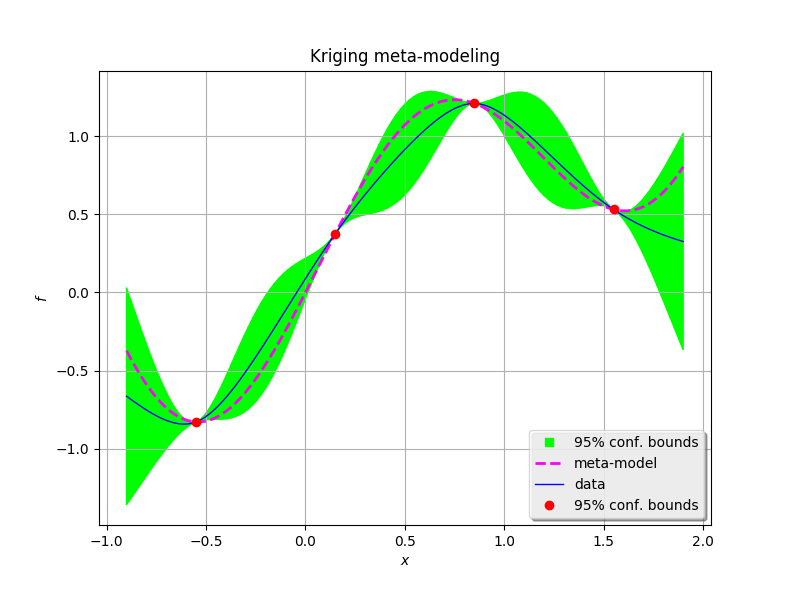
\includegraphics[width=0.2\textwidth]{figures/plot_kriging.png}&
  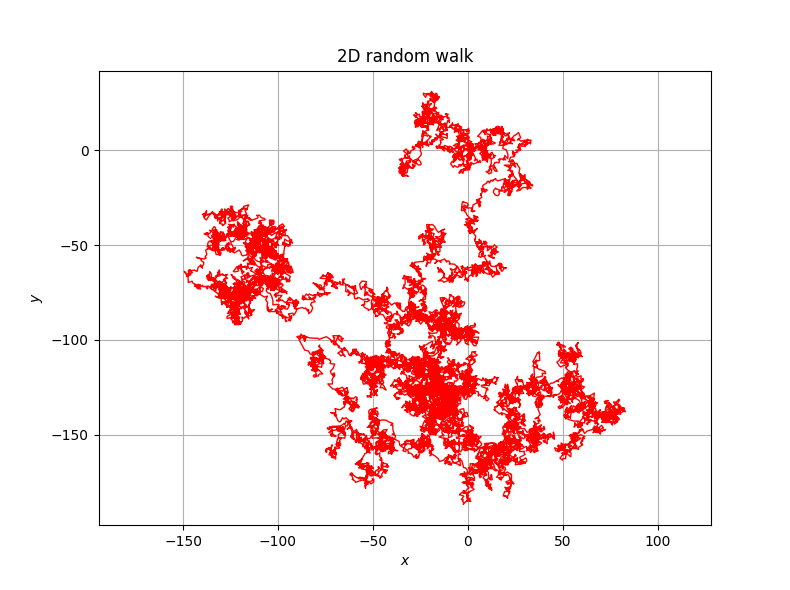
\includegraphics[width=0.2\textwidth]{figures/plot_random_walk.png}&
  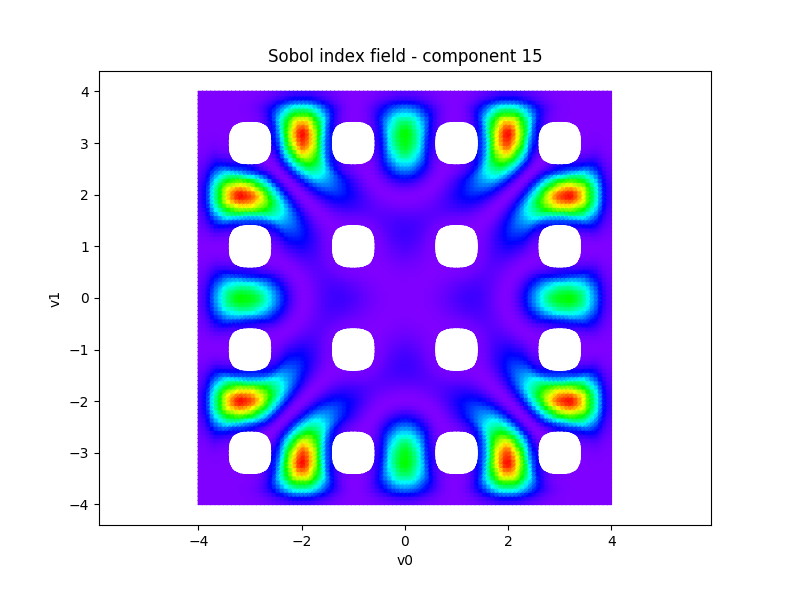
\includegraphics[width=0.2\textwidth]{figures/plot_sobol_field.png}&
  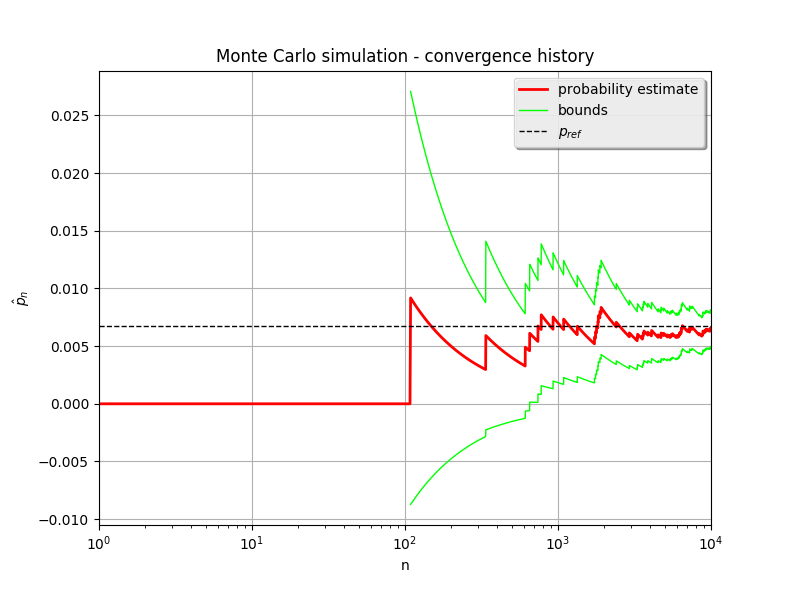
\includegraphics[width=0.2\textwidth]{figures/plot_monte_carlo.png}&
  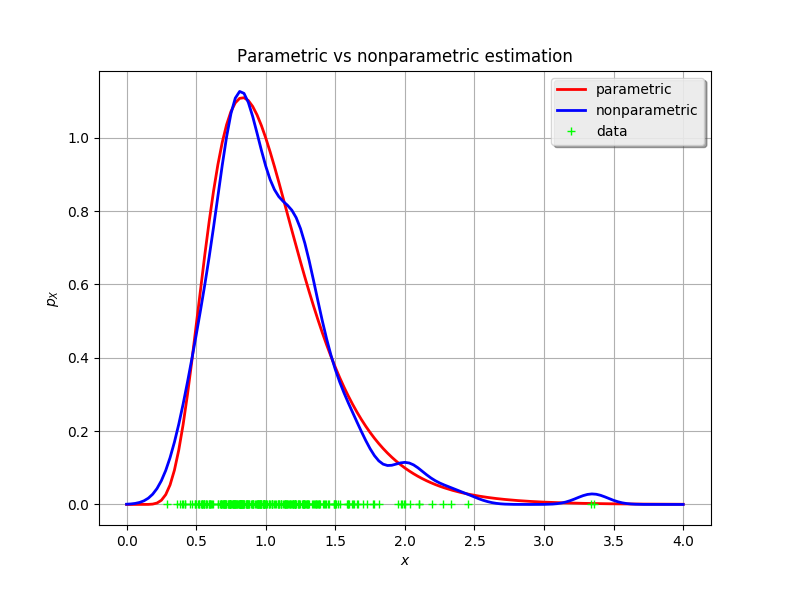
\includegraphics[width=0.2\textwidth]{figures/plot_distribution_fitting.png}
  \end{tabular}
\end{frame}
  

%%%%%%%%%%%%%%%%%%%%%%%%%%%%%%%%%%%%%%%%%%%%%%%%%%%%%%%%%%%%%%%%%%%%%%%%%%%%%

\begin{frame}[containsverbatim]
  \frametitle{OpenTURNS: documentation}
  
  \small{
  
  \begin{columns}
      \column{0.5\textwidth}
  
      \begin{center}
      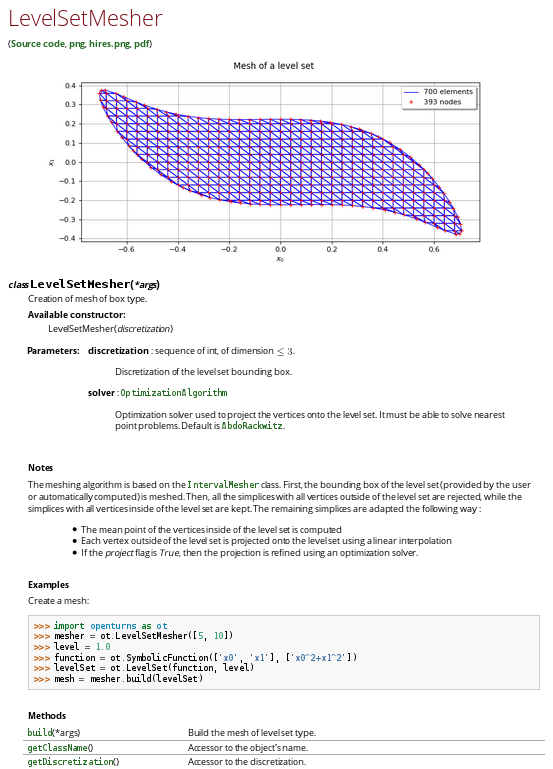
\includegraphics[width=0.8\textwidth]{figures/exClasses.png}
      \end{center}
  
      \column{0.5\textwidth}
  
    \begin{itemize}
    \item \underline{Content}: 
    \begin{itemize}
    \item Programming interface (API)
    \item Examples
    \item Theory
    \end{itemize}
    \item \emph{All} classes and methods 
    are documented, partly automatically.
    \item Examples are automatically tested at \emph{each} update 
    of the code and outputs are checked.
    \end{itemize}
    
  \end{columns}
  
  }
\end{frame}
  
%%%%%%%%%%%%%%%%%%%%%%%%%%%%%%%%%%%%%%%%%%%%%%%%%%%%%%%%%%%%%%%%%%%%%%%%%%%%%

\begin{frame}[containsverbatim]
  \frametitle{OpenTURNS: practical use}
  
  \small
  \begin{itemize}
  \item C++ and Python interface
  \vspace{10pt}
  \item Parallel computations with shared memory (TBB)
  \vspace{10pt}
  \item Optimized linear algebra with LAPACK and BLAS 
  \vspace{10pt}
  \item Possibility to interface with a computation cluster
  \vspace{10pt}
  \item Focused towards handling numerical data
  \vspace{10pt}
  \item Installation through conda, pip, packages for various Linux distros and source code
  \item 
  \begin{lstlisting}[language=Python, numbers = none]
import numpy as np
import openturns as ot
from openturns.viewer import View
ot.ResourceMap.SetAsString("Contour-DefaultColorMap", "viridis")
ot.ResourceMap.SetAsBool("Contour-DefaultIsFilled", True)
ot.ResourceMap.SetAsUnsignedInteger("Contour-DefaultLevelsNumber", 15)
\end{lstlisting}
  \end{itemize}


\end{frame}
  

%%%%%%%%%%%%%%%%%%%%%%%%%%%%%%%%%%%%%%%%%%%%%%%%%%%%%%%%%%%%%%%%%%%%%%%%%%%%%

\begin{frame}[containsverbatim]
  \frametitle{Coupling OpenTURNS with computer codes}
  
  \small
  
  OpenTURNS provides a text file exchange based interface in order to perform analyses on complex computer codes
  
  \vspace{10pt}
  
  \begin{columns}
      \column{0.6\textwidth}
      
  \centering
  
  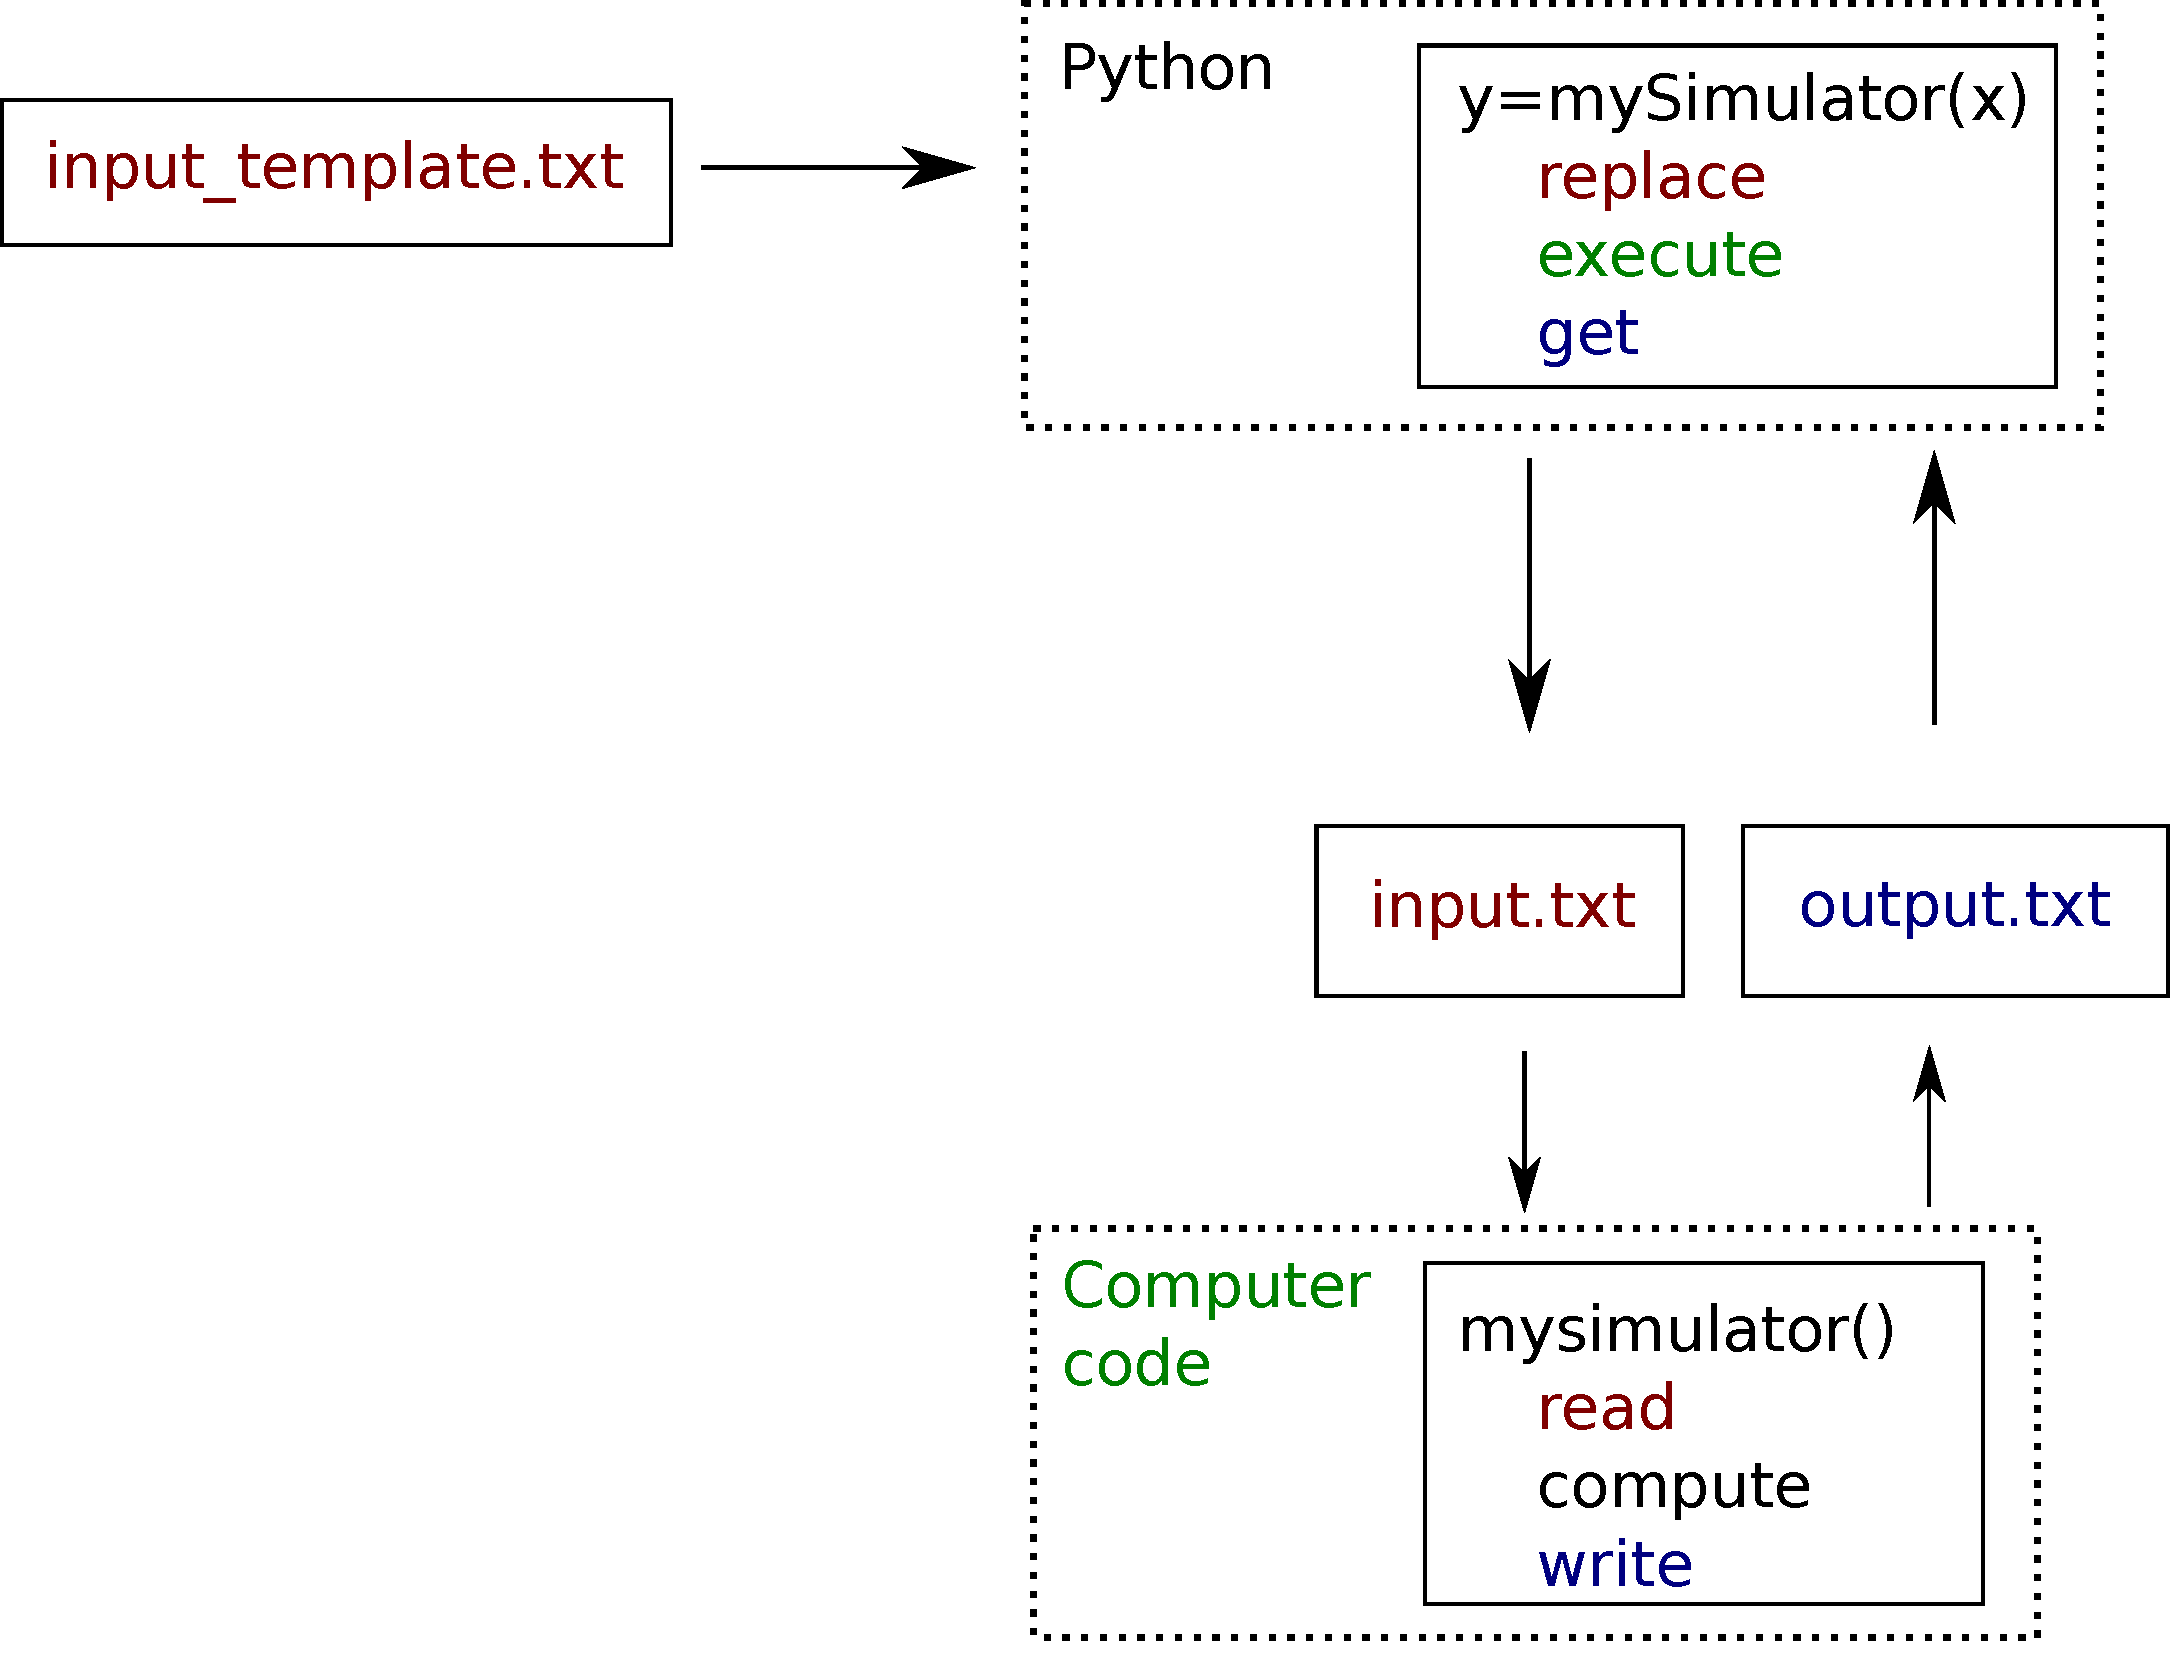
\includegraphics[width=1.\textwidth]{figures/Coupling.pdf}
  
      \column{0.4\textwidth}
  
  \begin{itemize}
  \item Replaces the need for input/output text parsers
  \item Wraps a simulation code under the form of a standard python function
  \item Allows to interface OpenTURNS with a cluster
  \item \href{https://openturns.github.io/otwrapy/master/index.html}{otwrapy}: interfacing tool to allow easy parallelization
  \end{itemize}
  
  \end{columns}
  
\end{frame}

%%%%%%%%%%%%%%%%%%%%%%%%%%%%%%%%%%%%%%%%%%%%%%%%%%%%%%%%%
%%%%%%%%%% GENERAL OPENTURNS PRESENTATION %%%%%%%%%%%%%%%
%%%%%%%%%%%%%%%%%%%%%%%%%%%%%%%%%%%%%%%%%%%%%%%%%%%%%%%%%

\begin{frame}[containsverbatim]
\frametitle{Probabilistic modeling}

\scriptsize

\underline{Random variables distributions}: 

\tiny 


\begin{minipage}[t]{0.5\textwidth}

Q: Gumbel(scale=558, mode=1013)>0

    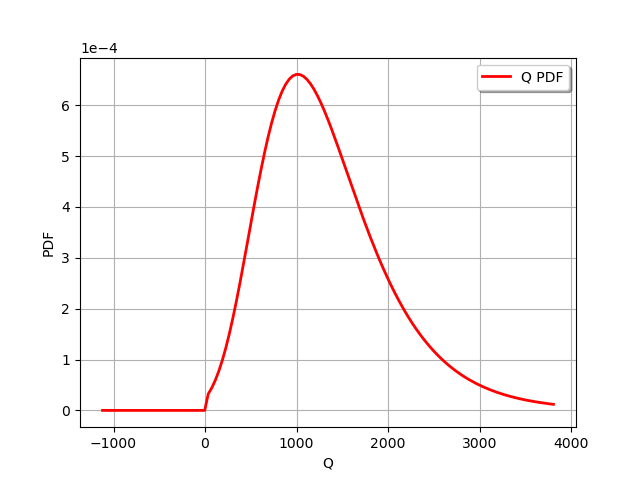
\includegraphics[width=.45\textwidth]{figures/Q.png}
    
\tiny
\begin{lstlisting}[language=Python]
d = ot.Gumbel(558.0, 1013.0)
tr = ot.TruncatedDistribution.LOWER
Q = ot.TruncatedDistribution(d, 0.0, tr)
\end{lstlisting}

\end{minipage}%
\begin{minipage}[t]{0.5\textwidth}

Ks: Normal(mean=30, std=7.5)>0

    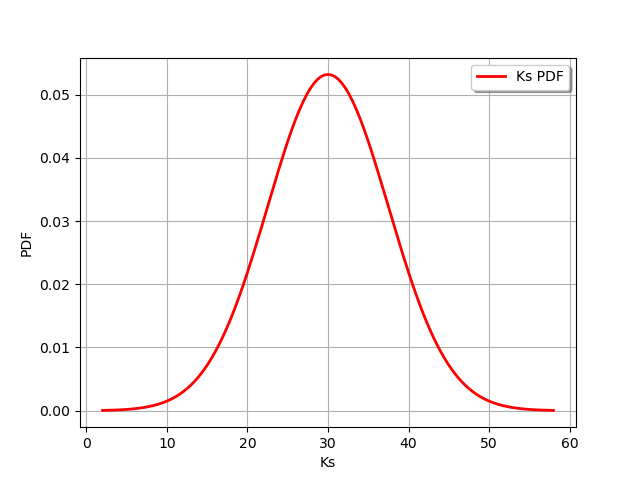
\includegraphics[width=.45\textwidth]{figures/Ks.png}
    
    \tiny
\begin{lstlisting}[language=Python]
d = ot.Normal(30.,7.5)
tr = ot.TruncatedDistribution.LOWER
Ks = ot.TruncatedDistribution(d, 0.0, tr)

\end{lstlisting}

\end{minipage}
\begin{minipage}[t]{0.5\textwidth}

Zv: Uniform(min=49, max=51)

    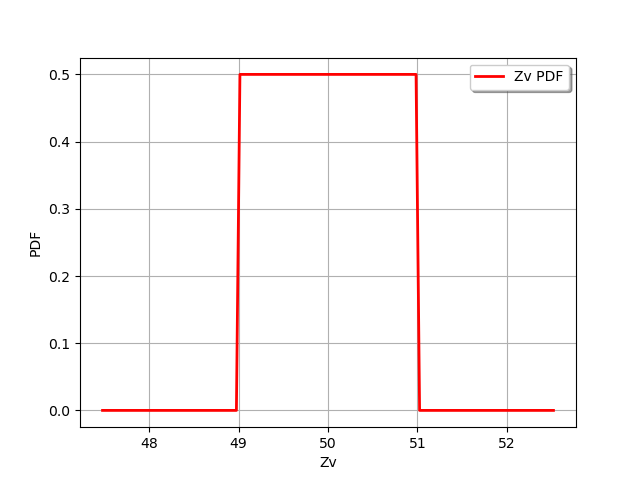
\includegraphics[width=.45\textwidth]{figures/Zv.png}
    
\end{minipage}%
\begin{minipage}[t]{0.5\textwidth}

Zm: Uniform(min=54, max=56)

    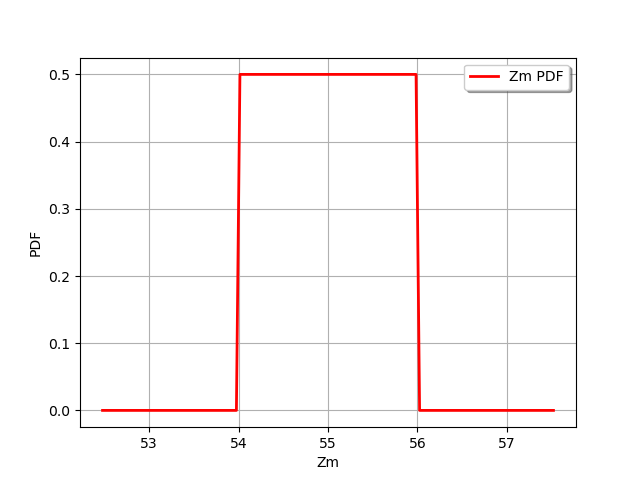
\includegraphics[width=.45\textwidth]{figures/Zm.png}
    
\end{minipage}%

\end{frame}


% %%%%%%%%%%%%%%%%%%%%%%%%%%%%%%%%%%%%%%%%%%%%%%%%%%%%%%%%%%%%%%%%%%%%%%%%%%%%%

\begin{frame}[containsverbatim]
\frametitle{Probabilistic modeling}

\scriptsize{

\begin{itemize}
\item We consider a 2-dimensional distribution with the following marginals: 
\begin{itemize}
\tiny
\item Gumbel(min = -1, max = 1)
\item Truncated normal (mean = 0, std = 1, min = -2, max = 2)
\end{itemize}
\end{itemize}

\begin{columns}
    \column{0.35\textwidth}

\underline{Marginals}

    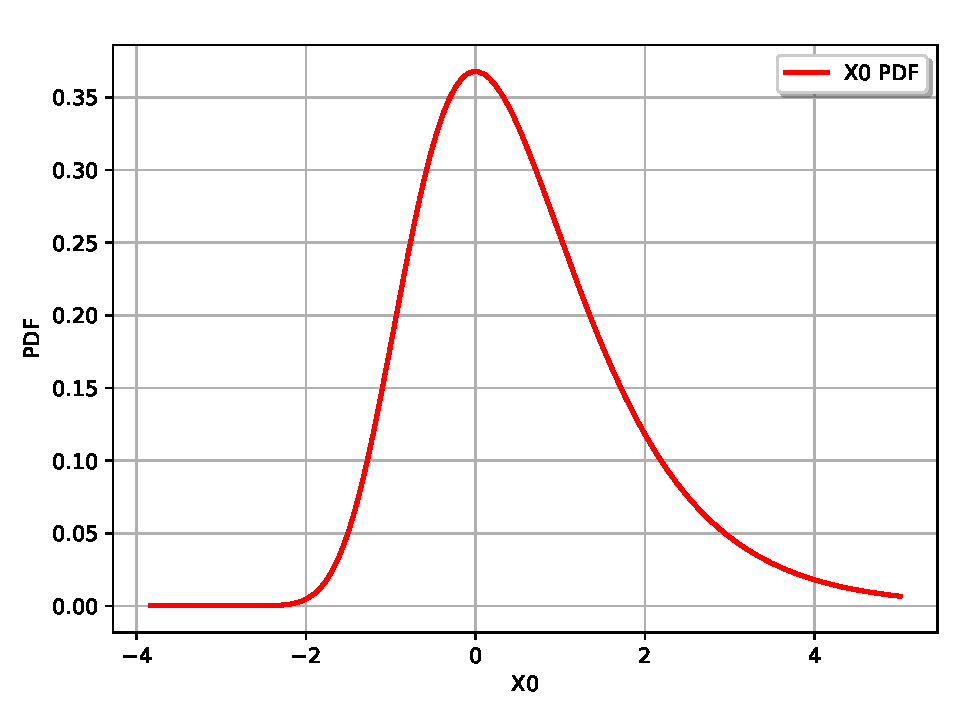
\includegraphics[width=0.8\textwidth]{figures/Marg1.pdf}

    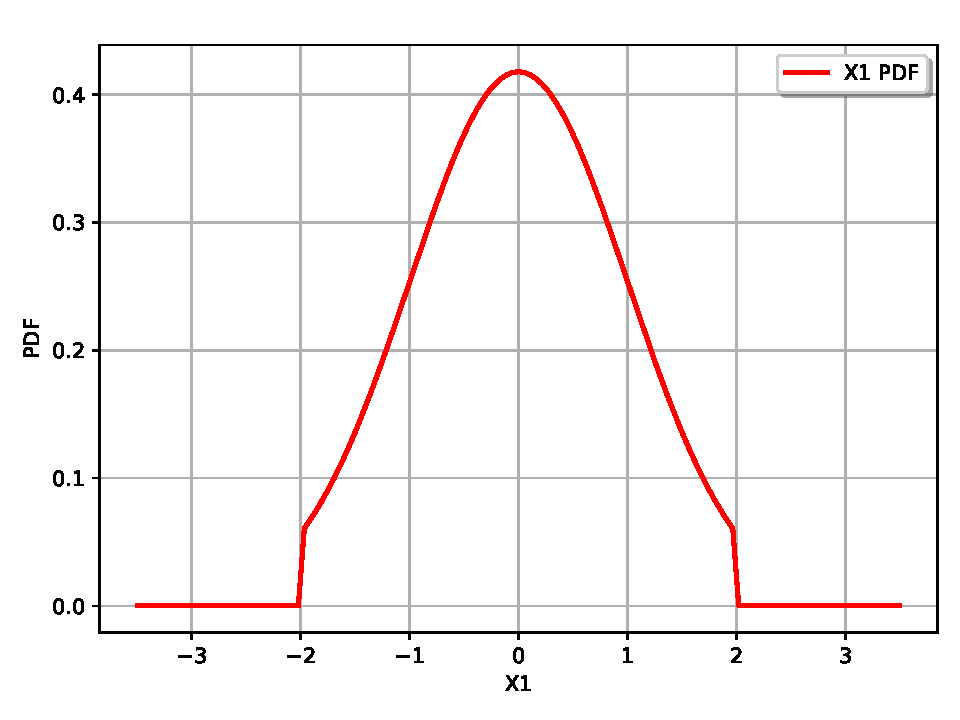
\includegraphics[width=0.8\textwidth]{figures/Marg2.pdf}


    \column{0.6\textwidth}
    
\underline{Joint distributions}

    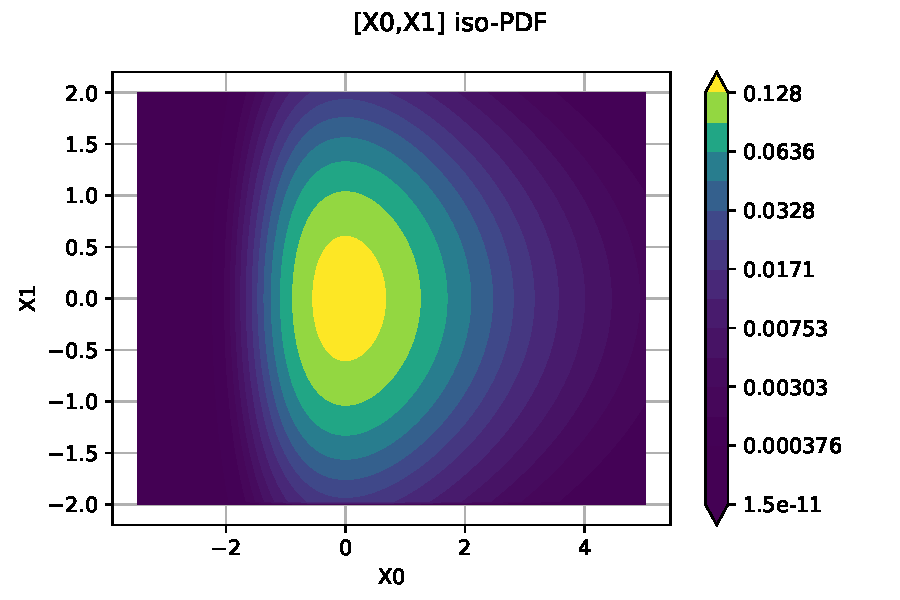
\includegraphics[width=\textwidth]{figures/Dist.pdf}

	
\end{columns}

}

\end{frame}


% %%%%%%%%%%%%%%%%%%%%%%%%%%%%%%%%%%%%%%%%%%%%%%%%%%%%%%%%%%%%%%%%%%%%%%%%%%%%%

\begin{frame}[containsverbatim]
\frametitle{Beyond independent marginals: Copulas}

\begin{minipage}[t]{0.5\textwidth}
    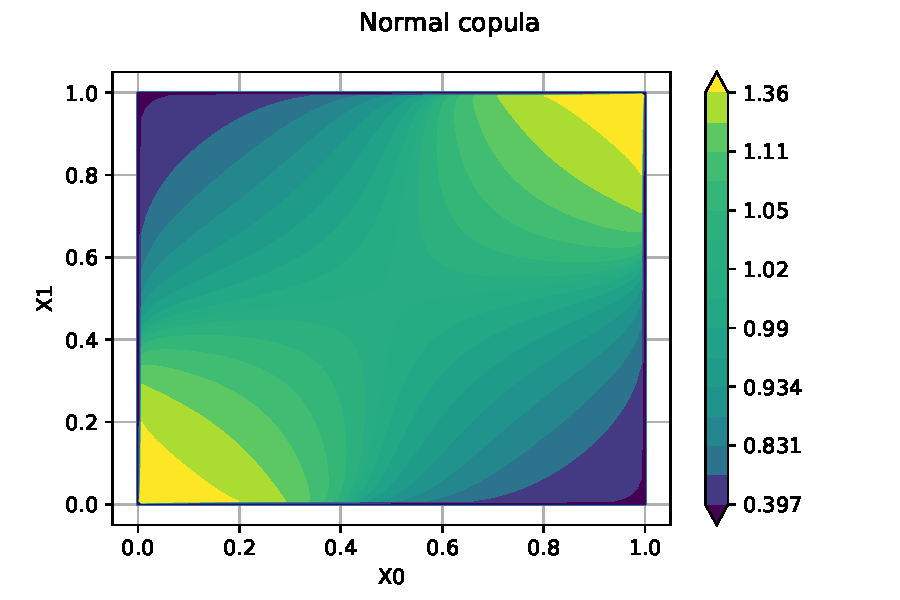
\includegraphics[width=.85\textwidth]{figures/Copula1.pdf}

\end{minipage}%
\begin{minipage}[t]{0.5\textwidth}
    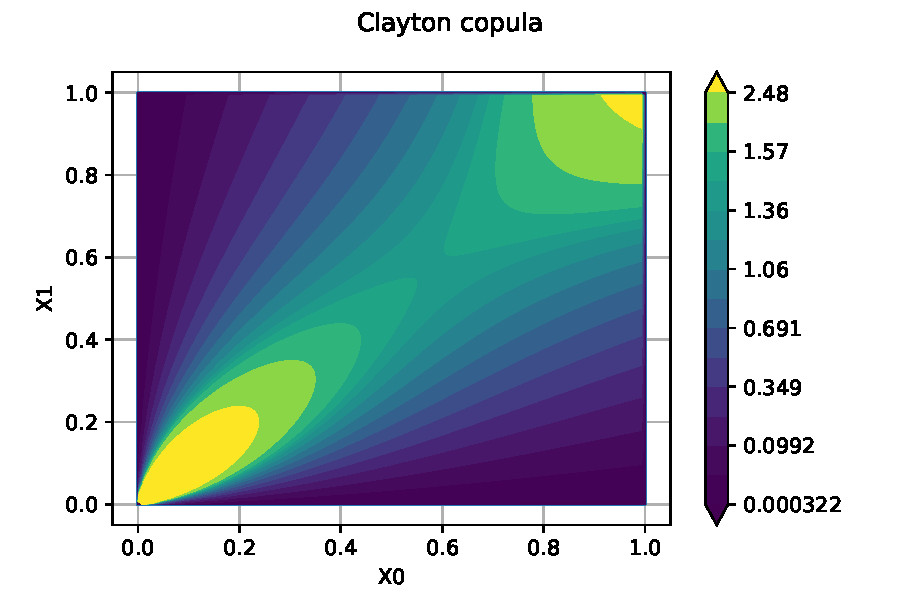
\includegraphics[width=.85\textwidth]{figures/Copula2.pdf}

\end{minipage}
\begin{minipage}[t]{0.5\textwidth}
    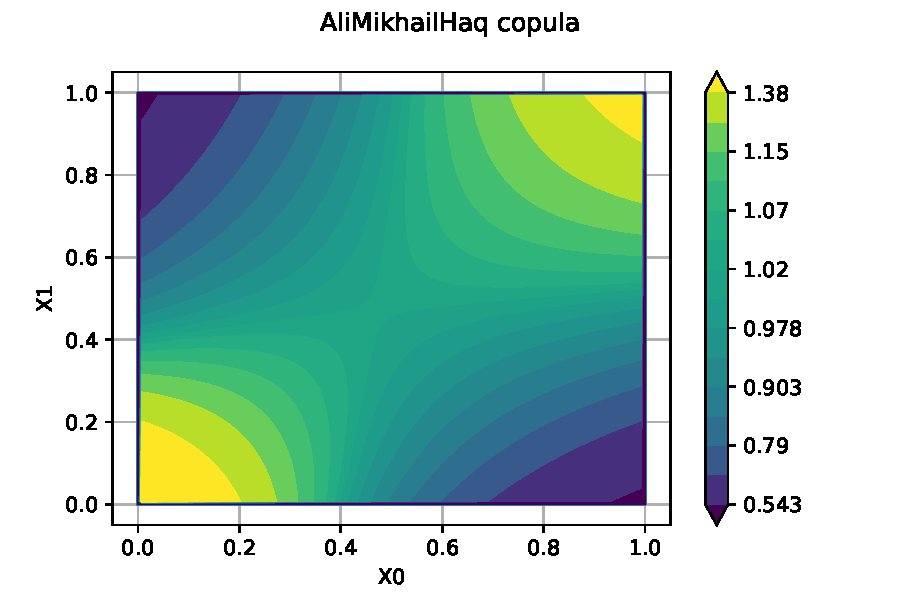
\includegraphics[width=.85\textwidth]{figures/Copula3.pdf}

\end{minipage}%
\begin{minipage}[t]{0.5\textwidth}
    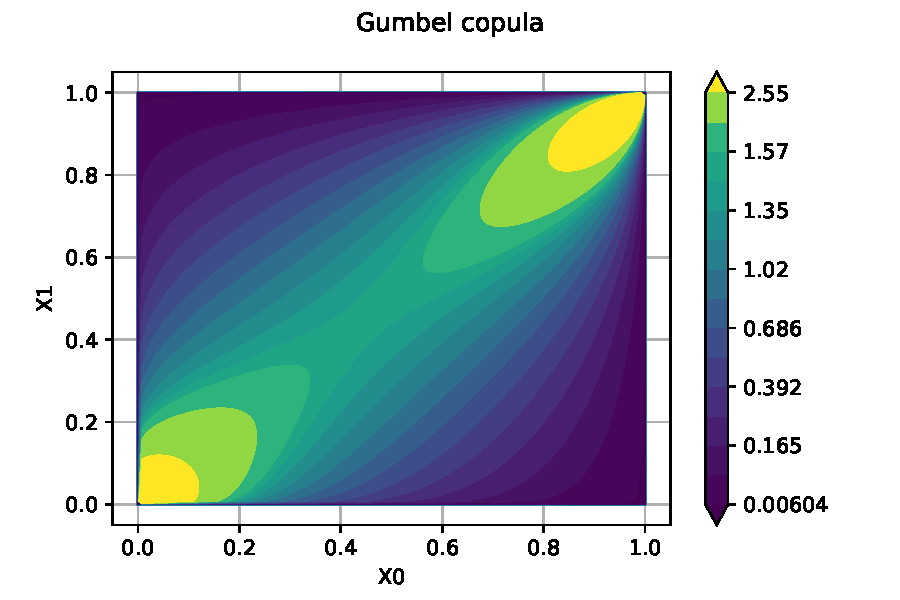
\includegraphics[width=.85\textwidth]{figures/Copula4.pdf}

\end{minipage}

\end{frame}


% %%%%%%%%%%%%%%%%%%%%%%%%%%%%%%%%%%%%%%%%%%%%%%%%%%%%%%%%%%%%%%%%%%%%%%%%%%%%%

\begin{frame}[containsverbatim]
\frametitle{Composing marginal distributions and copulas}

\begin{columns}
    \column{0.45\textwidth}

\begin{minipage}[t]{1.\textwidth}
    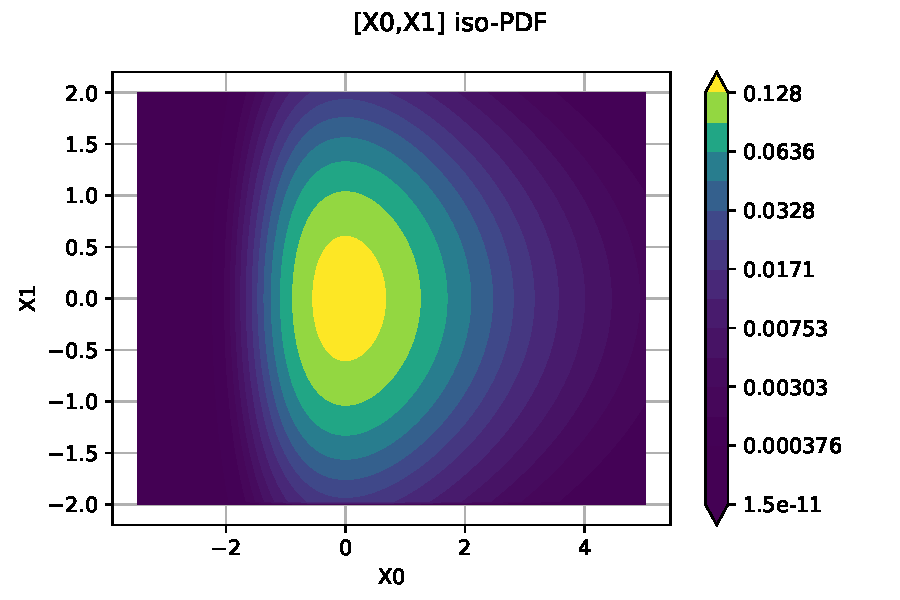
\includegraphics[width=.9\textwidth]{figures/Dist.pdf}

\end{minipage}

\begin{minipage}[t]{1.\textwidth}
    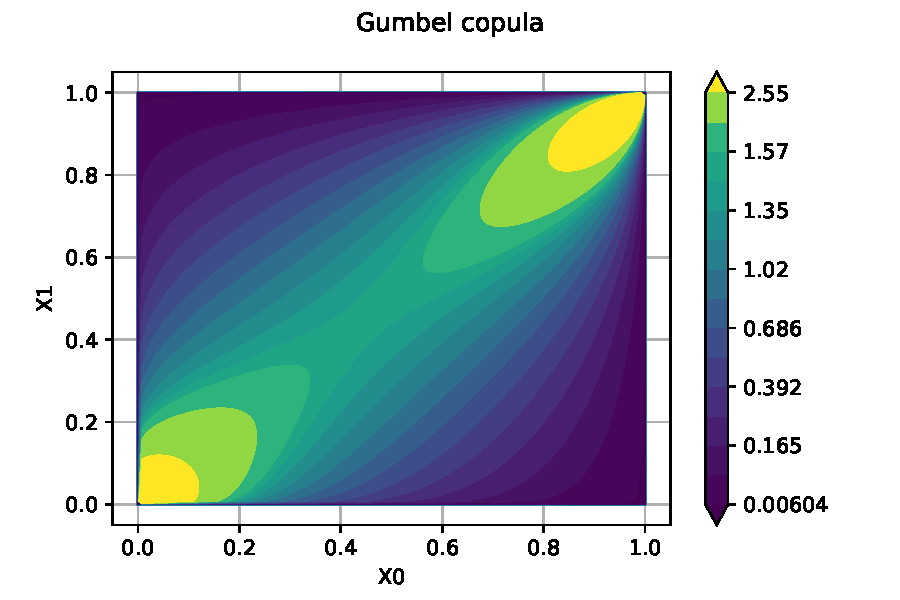
\includegraphics[width=.9\textwidth]{figures/Copula4.pdf}

\end{minipage}

    \column{0.55\textwidth}

\underline{We obtain:}
    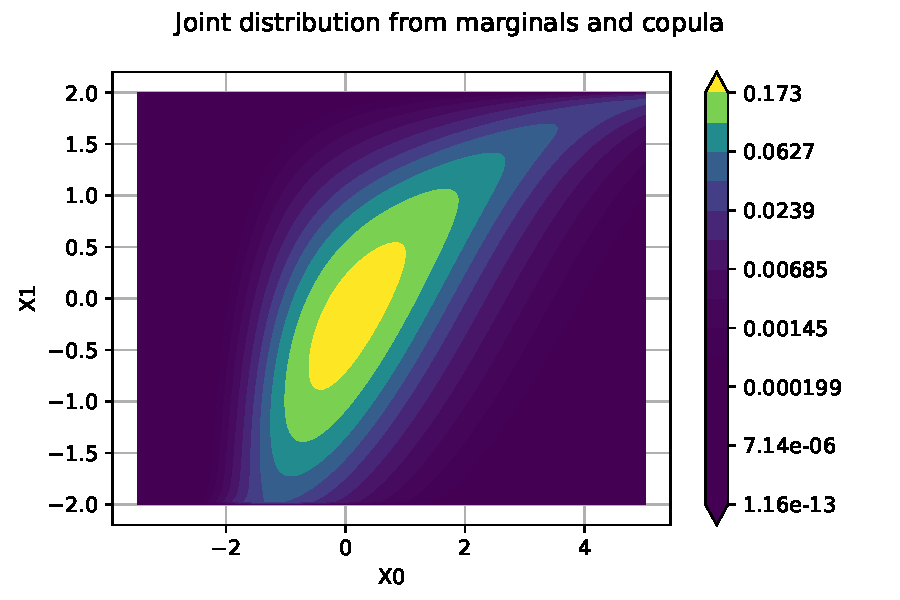
\includegraphics[width=\textwidth]{figures/ComposedGumbel.pdf}
    


\tiny
\begin{lstlisting}[language=Python, numbers = none]
marg1 = ot.Gumbel(1.0, 0.0)
marg2 = ot.TruncatedNormal(0.0, 1.0, -2.0, 2.0)
copula = ot.GumbelCopula()
joint = ot.JointDistribution([marg1, marg2], copula)
graph = joint.drawPDF()
title = "Joint distribution "
title += "from marginals and copula"
graph.setTitle(title)
\end{lstlisting}




\end{columns}


\end{frame}

%%%%%%%%%%%%%%%%%%%%%%%%%%%%%%%%%%%%%%%%%%%%%%%%%%%%%%%%%%%%%%%%%%%%%%%%%%%%%%

\begin{frame}[containsverbatim]
\frametitle{Design of experiments}

\scriptsize{

\begin{columns}
    \column{0.5\textwidth}

    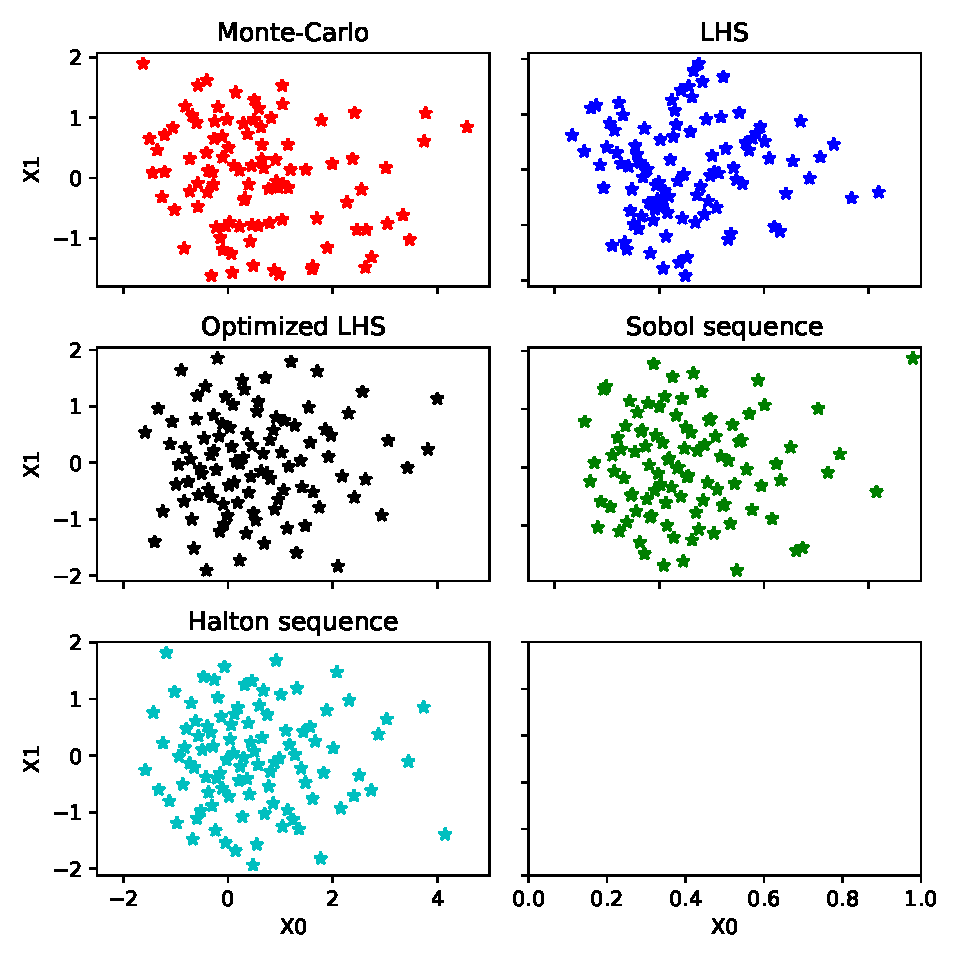
\includegraphics[width=1.\textwidth]{figures/DOE.pdf}

    \column{0.5\textwidth}
    
\tiny

\begin{lstlisting}[language=Python, numbers = none]
dim = 2
X=[ot.Gumbel(),ot.TruncatedNormal(0,1,-2,2)]
dist = ot.JointDistribution(X)
bounds = dist.getRange()
sampleSize = 100

sample1 = dist.getSample(sampleSize)

experiment = ot.LHSExperiment(dist,
	 sampleSize, False, False)
sample2 = experiment.generate()

lhs = ot.LHSExperiment(dist, sampleSize)
lhs.setAlwaysShuffle(True) # randomized
space_filling = ot.SpaceFillingC2()
temperatureProfile = ot.GeometricProfile(10.0, 0.95, 1000)
algo = ot.SimulatedAnnealingLHS(lhs, 
	space_filling, temperatureProfile)
sample3 = algo.generate()

sequence = ot.SobolSequence(dim) # or Halton
experiment = ot.LowDiscrepancyExperiment(
  sequence, dist, sampleSize, False)
sample4 = experiment.generate()

\end{lstlisting}
	
\end{columns}

}

\end{frame}



% %%%%%%%%%%%%%%%%%%%%%%%%%%%%%%%%%%%%%%%%%%%%%%%%%%%%%%%%%%%%%%%%%%%%%%%%%%%%%

\begin{frame}[containsverbatim]
\frametitle{Monte-Carlo sampling}

\scriptsize{

\begin{columns}
    \column{0.4\textwidth}

\begin{itemize}
\item The input distribution and relative output value are evaluated 10000 times
\item The output distribution can be infered as a parametric function or through histogram or kernel smoothing methods
\end{itemize}

    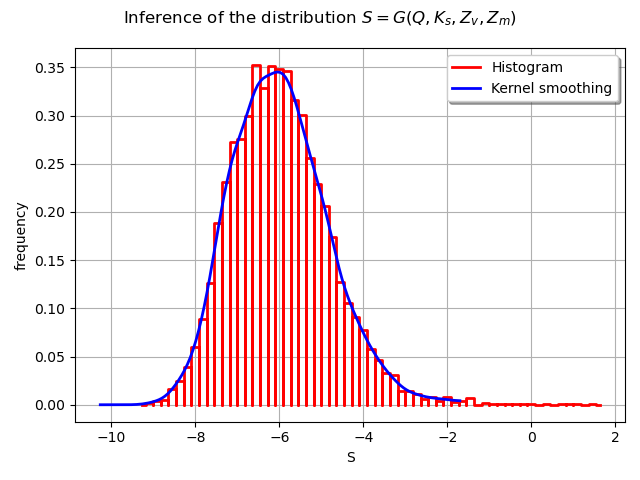
\includegraphics[width=1.\textwidth]{figures/S.png}

    \column{0.6\textwidth}
    
\tiny 
\begin{lstlisting}[language=Python, numbers = none]
Distribution = ot.JointDistribution([Q,Ks,Zv,Zm])

#Python model
def floodFunction(X):
    Q, Ks, Zv, Zm = X
    alpha = (Zm - Zv)/5.0e3
    H = (Q/(300.0*Ks*np.sqrt(alpha)))**0.6
    S = [H + Zv - 58.5]
    return S

fun = ot.PythonFunction(4,1,floodFunction)

#We define the output as a random vector
inputVector = ot.RandomVector(Distribution)
outputVector = ot.CompositeRandomVector(fun, inputVector)

#We sample and infere the output distribution
size = 10000
sampleY = outputVector.getSample(size)
hist = ot.HistogramFactory().build(sampleY)
graph = hist.drawPDF()
loiKS = ot.KernelSmoothing().build(sampleY)
graph2 = loiKS.drawPDF()

\end{lstlisting}

	
\end{columns}


}



\end{frame}

% %%%%%%%%%%%%%%%%%%%%%%%%%%%%%%%%%%%%%%%%%%%%%%%%%%%%%%%%%%%%%%%%%%%%%%%%%%%%%

\begin{frame}[containsverbatim]
\frametitle{Distribution and dependence inference}

\scriptsize{

\begin{columns}
    \column{0.6\textwidth}

    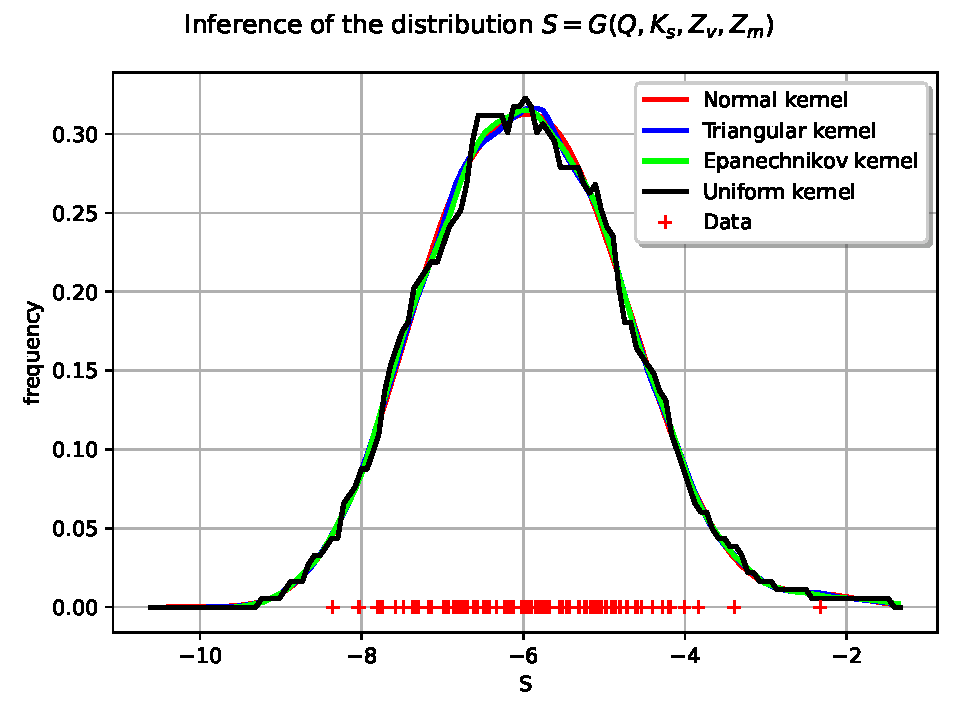
\includegraphics[width=.8\textwidth]{figures/Inference.pdf}


  
    \column{0.4\textwidth}
    

\scriptsize 
\begin{lstlisting}[language=Python, numbers = none]
size = 100
sampleY = outputVector.getSample(size)
graph = ot.KernelSmoothing(ot.Normal()).build(sampleY).drawPDF()
loiKS = ot.KernelSmoothing(ot.Triangular()).build(sampleY)
graph2 = loiKS.drawPDF()
graph.add(graph2)
loiKS = ot.KernelSmoothing(ot.Epanechnikov()).build(sampleY)
graph2 = loiKS.drawPDF()
graph.add(graph2)
loiKS = ot.KernelSmoothing(ot.Uniform()).build(sampleY)
graph2 = loiKS.drawPDF()

\end{lstlisting}

	  \begin{itemize}
  \item Parametric ($1d - Nd$) distribution inference
  \item Non-parametric ($1d - Nd$) distribution inference
  \item Parametric copula inference
  \item Non-parametric copula inference (Bernstein copula)
  \item Resampling w.r.t. inferred distributions
  \end{itemize}
  
\end{columns}


}


\end{frame}

% %%%%%%%%%%%%%%%%%%%%%%%%%%%%%%%%%%%%%%%%%%%%%%%%%%%%%%%%%%%%%%%%%%%%%%%%%%%%%

\begin{frame}[containsverbatim]
\frametitle{Iterative Monte-Carlo: Central tendency anaysis}

\scriptsize{

\begin{columns}
    \column{0.44\textwidth}

\begin{itemize}
\item The expected value and associated standard deviation are computed iteratively
\item Different stopping criteria can be used 
\item Batch computation can be used
\end{itemize}

    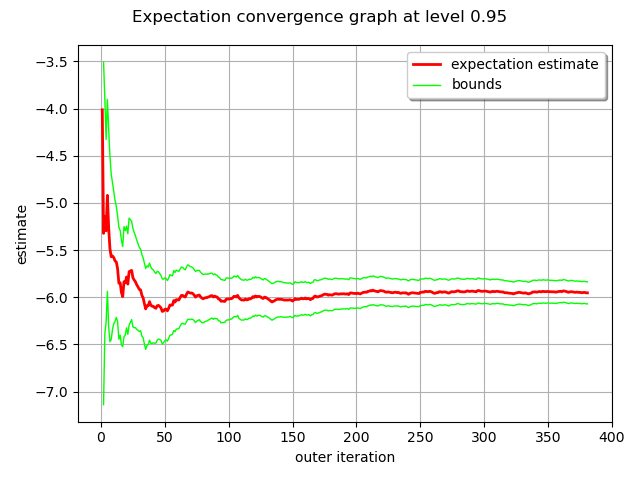
\includegraphics[width=.95\textwidth]{figures/Expectation.png}

    \column{0.56\textwidth}
    
 \footnotesize
\begin{eqnarray*}
\widehat{m}_y & = & \frac{1}{N}\sum_1^N G(\mathbf{X}_i) \\
\widehat{\sigma}_y  & = & \sqrt{\frac{1}{N}\sum_1^N (G(\mathbf{X}_i)-\hat{m}_y)^2} \\
\widehat{\sigma}_{m_y} & = & \widehat{\sigma}_y / \sqrt{N}
\end{eqnarray*}


\tiny 
\begin{lstlisting}[language=Python, numbers = none]
algo = ot.ExpectationSimulationAlgorithm(outputVector)
algo.setMaximumOuterSampling(100000)
algo.setBlockSize(1)
algo.setCoefficientOfVariationCriterionType("MAX")
algo.setMaximumCoefficientOfVariation(0.01)
algo.run()
graph = algo.drawExpectationConvergence()
\end{lstlisting}

	
\end{columns}

}

\end{frame}

% %%%%%%%%%%%%%%%%%%%%%%%%%%%%%%%%%%%%%%%%%%%%%%%%%%%%%%%%%%%%%%%%%%%%%%%%%%%%%

\begin{frame}[containsverbatim]
\frametitle{Iterative Monte-Carlo: Reliability analysis}

\scriptsize{

\begin{columns}
    \column{0.5\textwidth}

\begin{itemize}
\item We now consider the probability of flooding:  ($P(S>0.)$) 
\item Same as before, but the function $\mathbb{I}_{G(\mathbf{X}_i)>0} $ is considered
\end{itemize}

    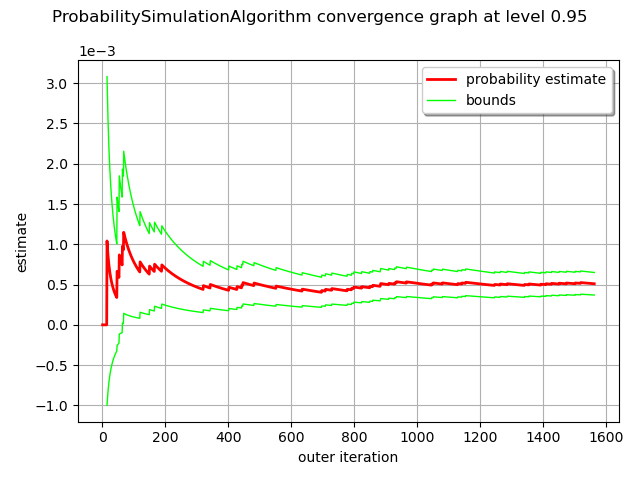
\includegraphics[width=1.\textwidth]{figures/Probability.png}

    \column{0.5\textwidth}
 
    
 \footnotesize
\begin{eqnarray*}
\widehat{p}_y & = & \frac{1}{N}\sum_1^N \mathbb{I}_{G(\mathbf{X}_i)>0} \\
\widehat{\sigma}  & = & \sqrt{\frac{1}{N}\sum_1^N (\mathbb{I}_{G(\mathbf{X}_i)>0}-\hat{p}_y)^2} \\
\widehat{\sigma}_{p_y} & = & \widehat{\sigma} / \sqrt{N}
\end{eqnarray*}

\tiny 
\begin{lstlisting}[language=Python, numbers = none]

eventF = ot.ThresholdEvent(outputVector, ot.GreaterOrEqual(), 0.0)
exp = ot.MonteCarloExperiment()
algo = ot.ProbabilitySimulationAlgorithm(eventF, exp)
algo.setMaximumOuterSampling(100000)
algo.setMaximumCoefficientOfVariation(0.01)
algo.setBlockSize(10)
algo.run()


\end{lstlisting}

	
\end{columns}

}

\end{frame}


% %%%%%%%%%%%%%%%%%%%%%%%%%%%%%%%%%%%%%%%%%%%%%%%%%%%%%%%%%%%%%%%%%%%%%%%%%%%%%

\begin{frame}[containsverbatim]
\frametitle{FORM/SORM reliability analysis}

\scriptsize{

\begin{columns}
    \column{0.5\textwidth}

\begin{itemize}

\item We estimate the probability of flooding through FORM/SORM procedures

\vspace{10pt}

\item MC estimation requires $\simeq$ 1500 function evaluations 
\item FORM and SORM only use $\simeq 150$
\end{itemize}

\begin{block}{}
\begin{itemize}
\item Estimated probability:
\begin{itemize}
\tiny
\item MC: 5.09999999999998 1e-4
\item FORM: 5.340929030055227 1e-4
\item SORM: 6.793780433482759 1e-4
\end{itemize}
\end{itemize}
\end{block}

    \column{0.5\textwidth}
    
\tiny 
\begin{lstlisting}[language=Python, numbers = none]
#FORM
OptAlgo = ot.Cobyla()
startingPoint = Distribution.getMean()
algoFORM = ot.FORM(OptAlgo, eventF, 
startingPoint)
algoFORM.run()

#SORM
OptAlgo = ot.Cobyla()
startingPoint = Distribution.getMean()
algoSORM = ot.SORM(OptAlgo, eventF, 
startingPoint)
algoSORM.run()
\end{lstlisting}

\scriptsize

\vspace{20pt}

\textcolor{red}{Different types and parameterizations of finite difference gradient computation are available}

\end{columns}

\textbf{Also:}

\begin{itemize}
\item Directional sampling
\item Importance sampling (FORM-IS, NAIS, Adaptive IS-Cross-entropy)
\item Subset sampling
\end{itemize}
}

\end{frame}


% %%%%%%%%%%%%%%%%%%%%%%%%%%%%%%%%%%%%%%%%%%%%%%%%%%%%%%%%%%%%%%%%%%%%%%%%%%%%%



\begin{frame}
\frametitle{Sensitivity analysis}

\begin{minipage}[c]{0.6\textwidth}


Various sensitivity analysis methods are available
\begin{itemize}
\item Graphical analysis
\begin{itemize}
\item Pair plots
\item Parallel coordinates plots
\item Cross-cuts
\end{itemize}
\vspace{15pt}
\item Quantitative indices 
\begin{itemize}
\item SRC, SRRC, PRC, PRCC
\item Sobol' indices (multiple estimators)
\item FAST indices
\item ANCOVA indices
\item HSIC indices
\item Shapley Indices (available as a module)

\end{itemize}
\end{itemize}

\end{minipage}%
\begin{minipage}[c]{0.45\textwidth}
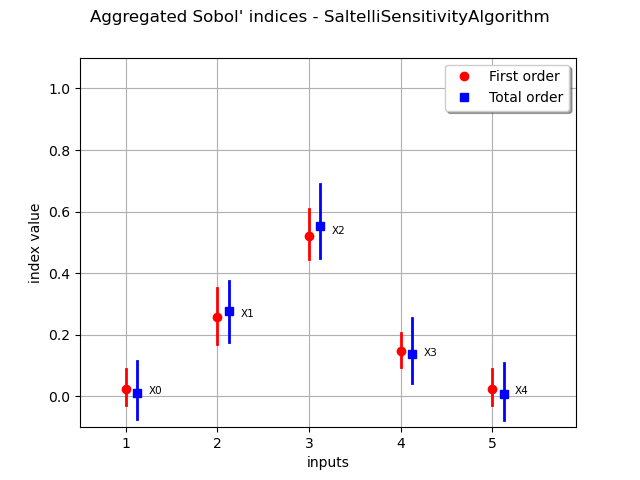
\includegraphics[width=1.\textwidth]{figures/SobolEx.png}
\end{minipage}

\end{frame}

% %%%%%%%%%%%%%%%%%%%%%%%%%%%%%%%%%%%%%%%%%%%%%%%%%%%%%%%%%%%%%%%%%%%%%%%%%%%%%



\begin{frame}
\frametitle{Sensitivity analysis: Parallel coordinates plot}

\centering
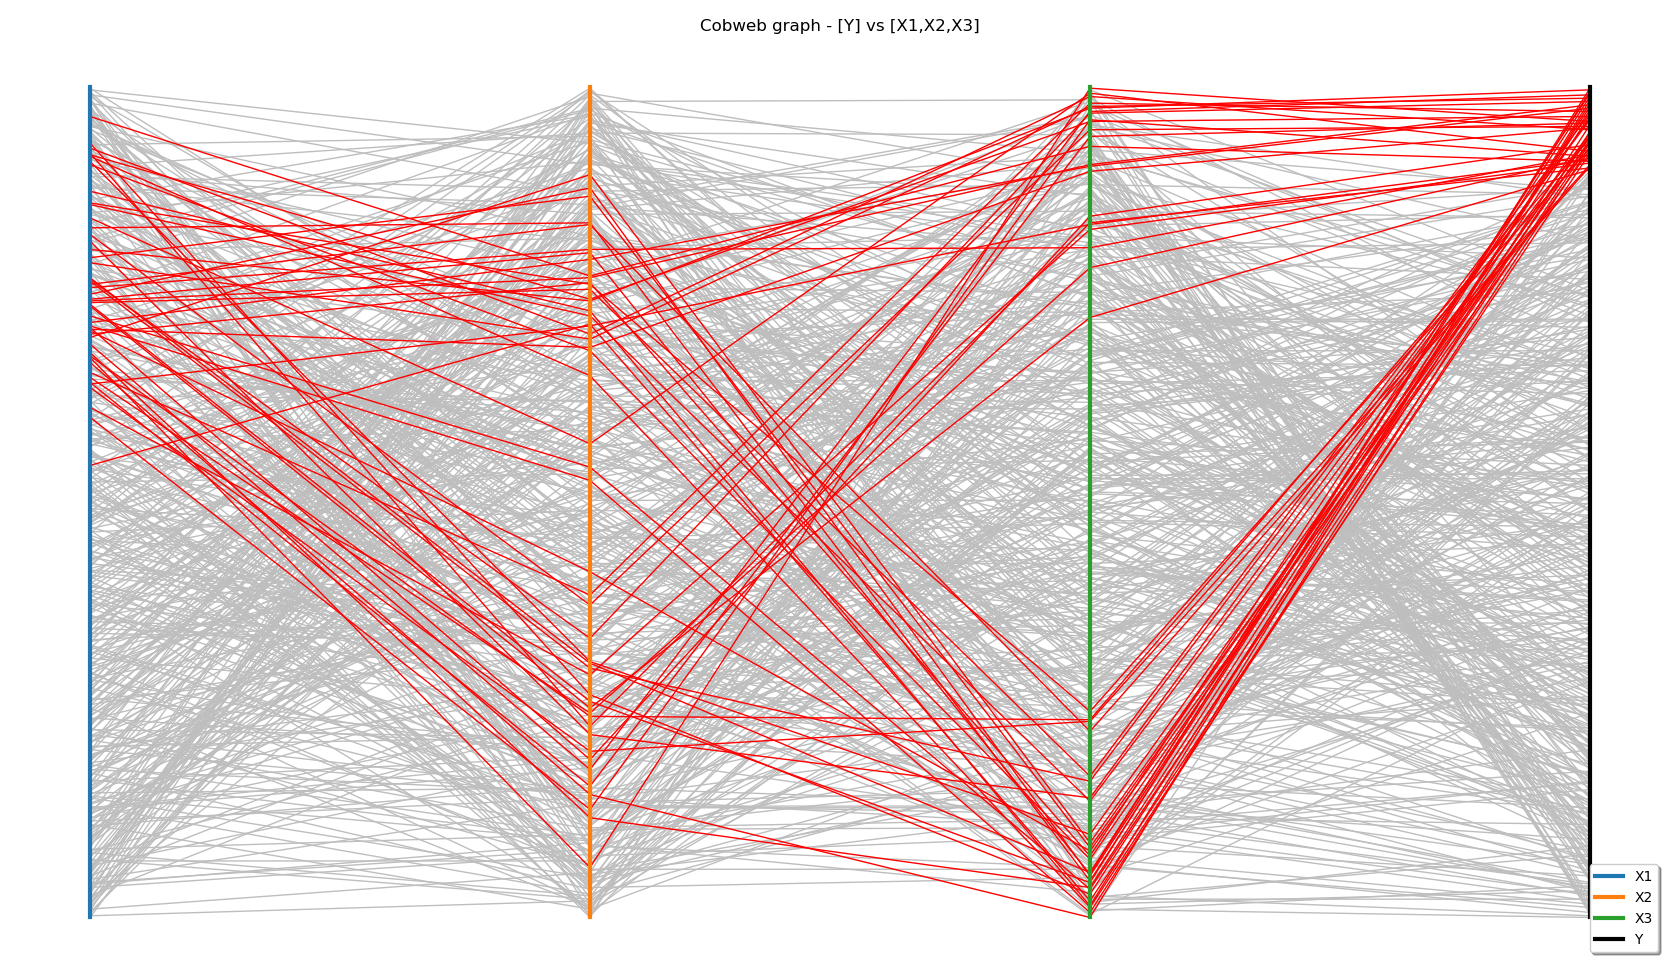
\includegraphics[width=.8\textwidth]{figures/CobwebOT.png}


\end{frame}

%********************************************************************%
\begin{frame}
\frametitle{Sensitivity analysis: HSIC indices and associated p-values}

  
  \begin{columns}
    \column{0.49\textwidth}
    
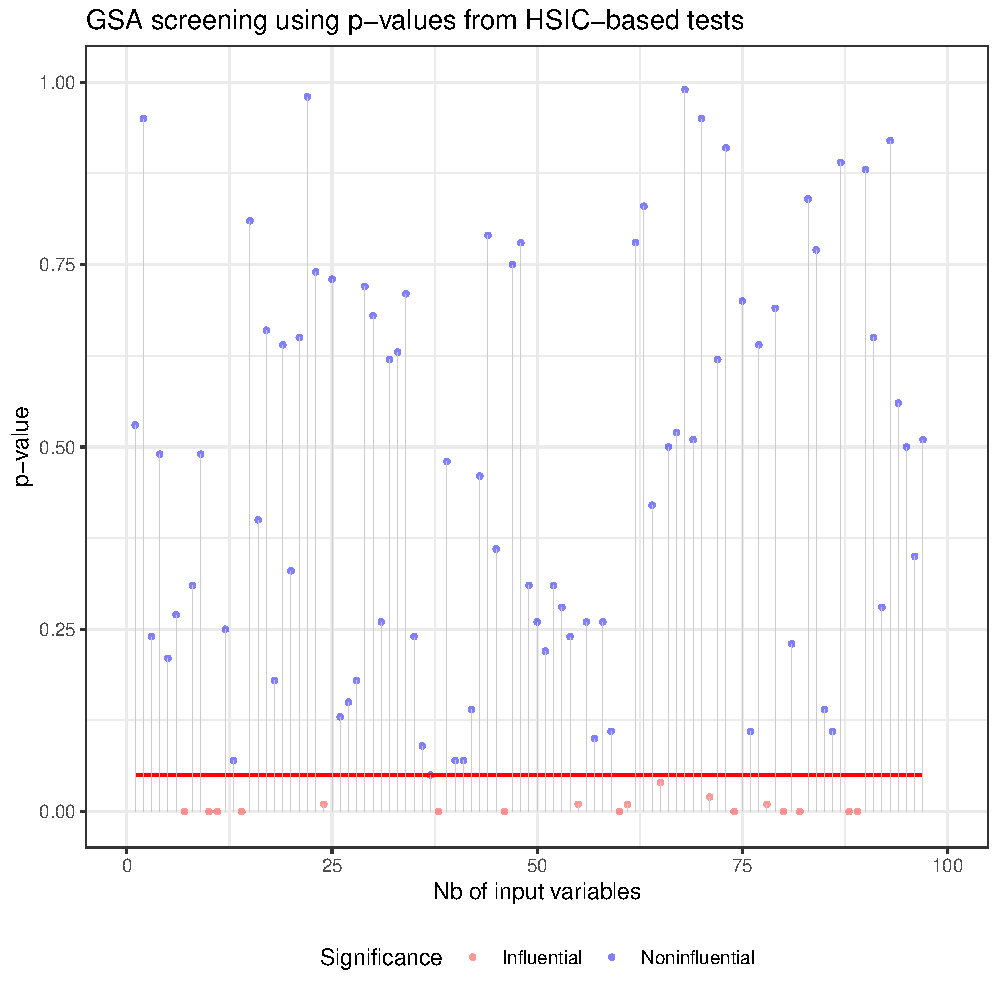
\includegraphics[width=.9\textwidth]{figures/plot_pval_GSA_MDTE.pdf}

\centering 
\small GSA-oriented screening.

    \column{0.49\textwidth}

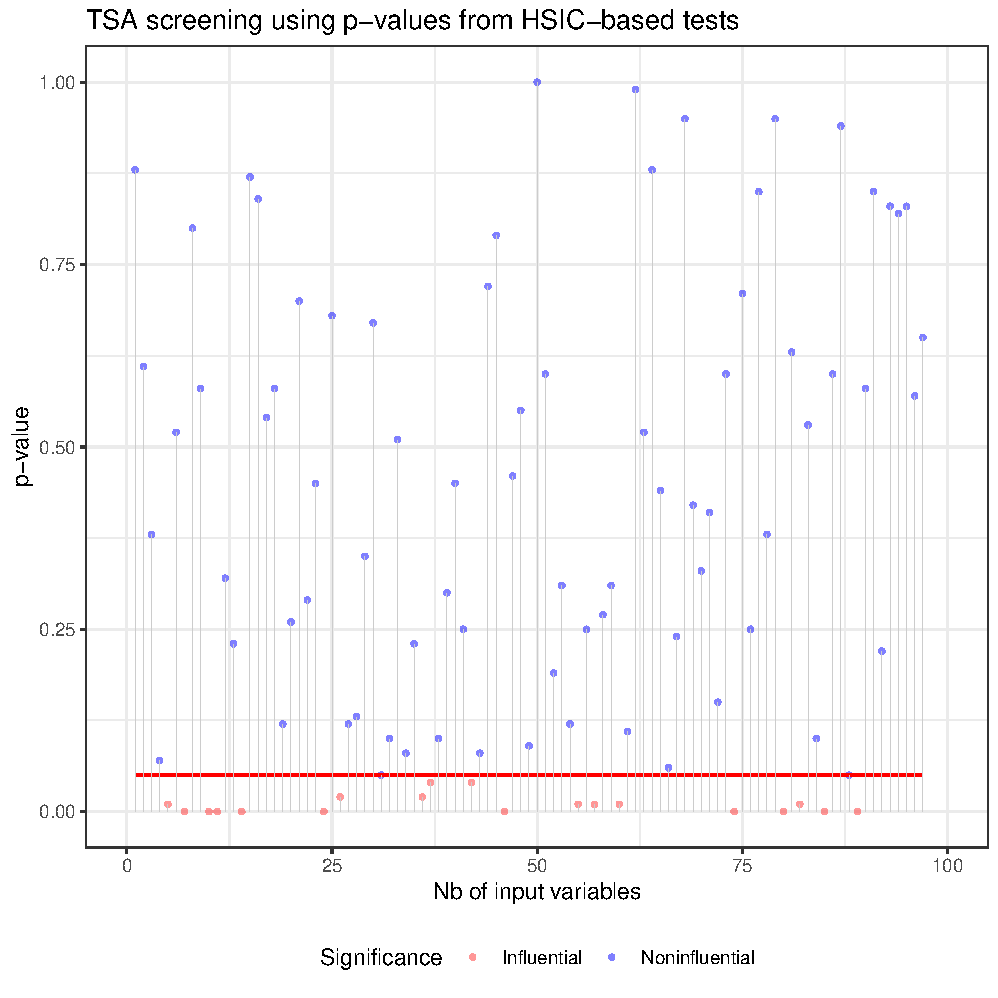
\includegraphics[width=.9\textwidth]{figures/plot_pval_TSA_MDTE.pdf}

\centering 
\small TSA-oriented screening.

\end{columns}


\end{frame}

%********************************************************************%



% %%%%%%%%%%%%%%%%%%%%%%%%%%%%%%%%%%%%%%%%%%%%%%%%%%%%%%%%%%%%%%%%%%%%%%%%%%%%%

\begin{frame}[containsverbatim]
\frametitle{Surrogate modeling: Gaussian process regression}

\begin{minipage}[t]{0.5\textwidth}
    
\small 
\begin{itemize}
\item Different surrogate modeling methods are available
\begin{itemize}
\tiny
\item Kriging
\item Polynomial chaos expansion
\item Linear regression \& step-wise basis selection
\item Low rank tensors
\item automatic validation tools
\end{itemize}
\end{itemize}



    
\centering
    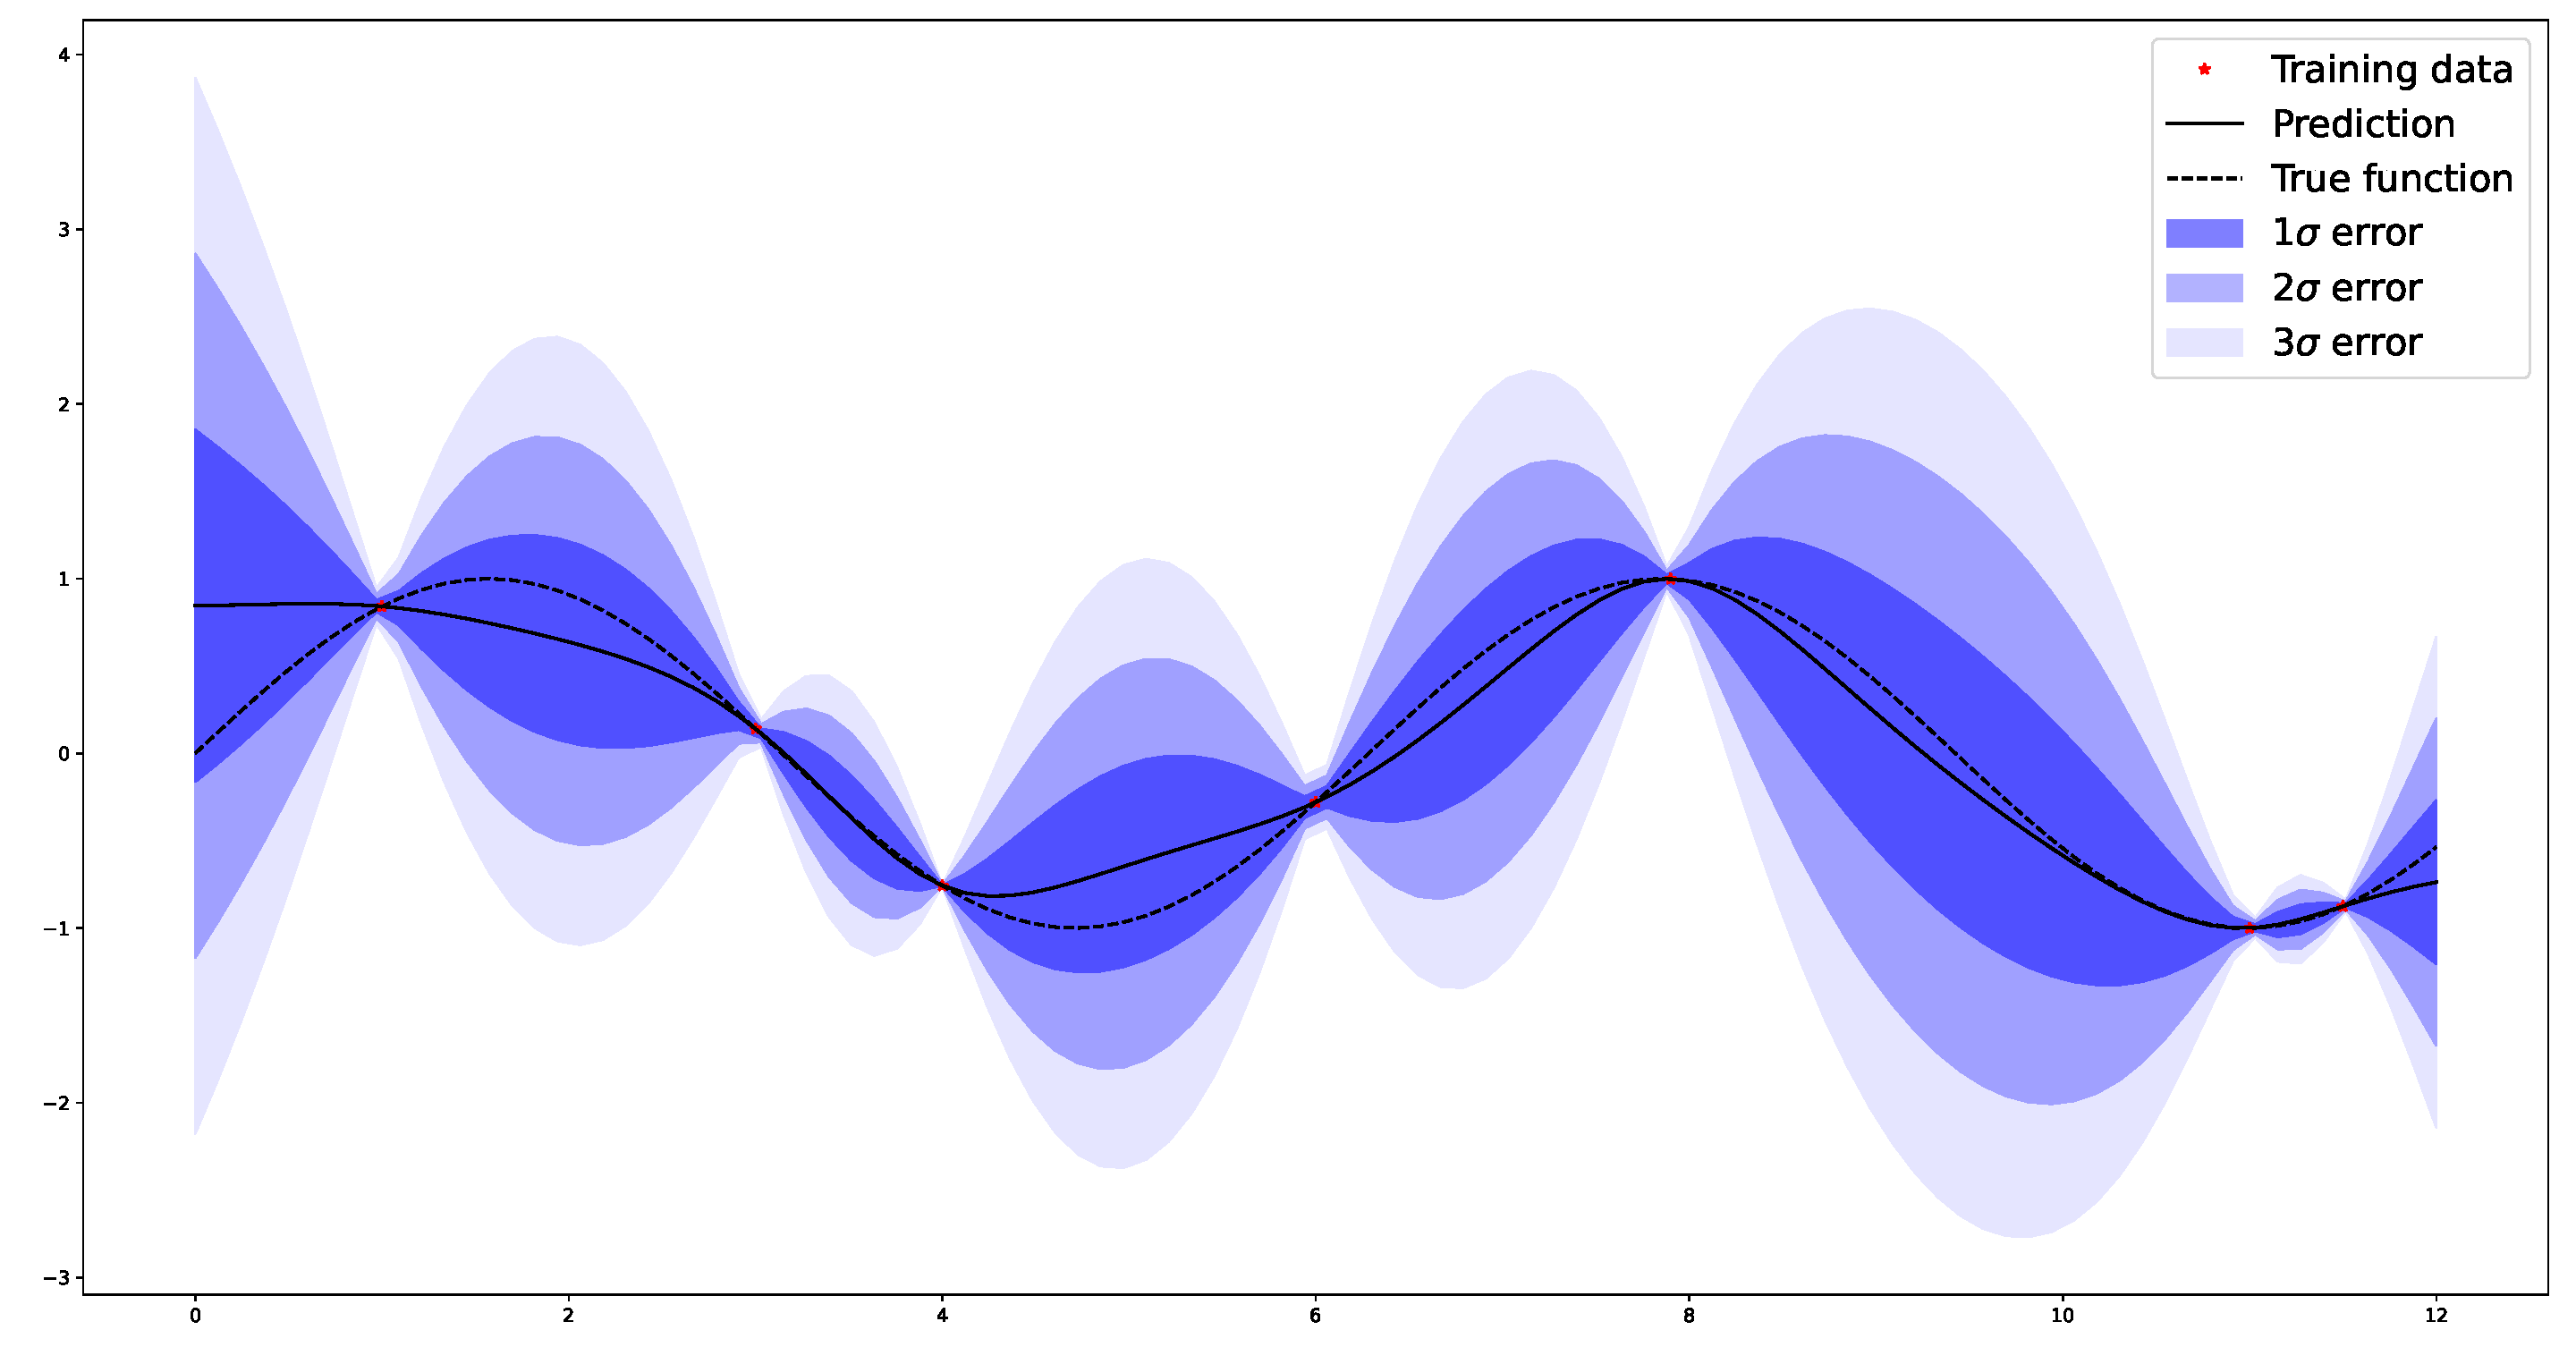
\includegraphics[width=.9\textwidth]{figures/Kriging.pdf}
    
\end{minipage}%
\begin{minipage}[t]{0.5\textwidth}
    
\small
\begin{itemize}
\item Gaussian process regression
\begin{itemize}
\tiny
\item Different types of covariance functions and function basis can be used
\item User-defined options are also available
\item MLE optimization can be parameterized
\item Large number of optimization algorithms available
\end{itemize}
\end{itemize}


\tiny
\begin{lstlisting}[language=Python, numbers = none]
inputSample = Distribution.getSample(100)
outputSample = fun(inputSample)

dimension = 4
basis = ot.ConstantBasisFactory(dimension).build()
covarianceModel = ot.SquaredExponential()

algo = ot.KrigingAlgorithm(inputSample, outputSample, covarianceModel, basis)
  
algo.run()
result = algo.getResult()
KrigingMM = result.getMetaModel()
\end{lstlisting}

\end{minipage}

\end{frame}



% %%%%%%%%%%%%%%%%%%%%%%%%%%%%%%%%%%%%%%%%%%%%%%%%%%%%%%%%%%%%%%%%%%%%%%%%%%%%%

\begin{frame}[containsverbatim]
\frametitle{Optimization}


\begin{itemize}
\item OpenTURNS provides an interface with several optimization libraries
\begin{itemize}
\item Bonmin
\item NLopt
\item dlib
\item pagmo
\end{itemize}

\item Ad-hoc implementation of the COBYLA algorithm

\vspace{6pt}


\item Constrained and unconstrained optimization
\item Gradient-based and derivative-free optimizaiton
\item Bounded and unbounded optimization
\item Single and multi-objective optimization
\item Multi-start wrapper


\end{itemize}


\end{frame}



% %%%%%%%%%%%%%%%%%%%%%%%%%%%%%%%%%%%%%%%%%%%%%%%%%%%%%%%%%%%%%%%%%%%%%%%%%%%%%

\begin{frame}[containsverbatim]
\frametitle{Field function modeling}

\scriptsize 
\begin{columns}
    \column{0.45\textwidth}

    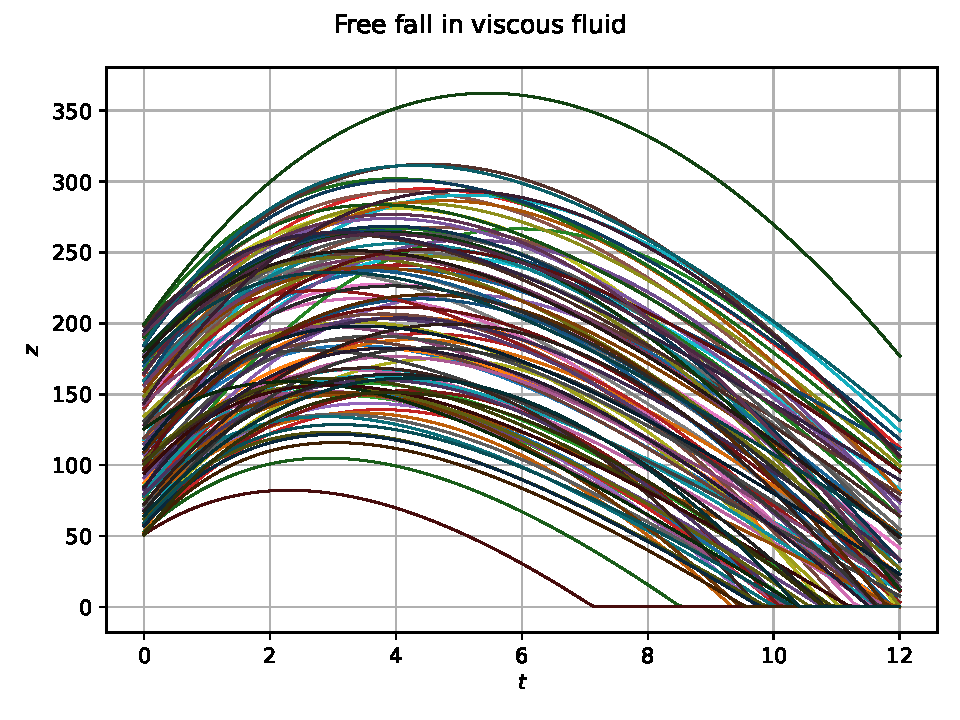
\includegraphics[width=1.\textwidth]{figures/Trajectories.pdf}
    
\column{0.55\textwidth}
        
\tiny
\begin{lstlisting}[language=Python, numbers = none]
def free_fall(X):
    g  = 9.81
    z0,v0,m,c = X
    tau=m/c
    vinf=-m*g/c
    t = np.array(mesh.getVertices().asPoint())
    z=z0+vinf*t+tau*(v0-vinf)*(1-np.exp(-t/tau))
    z=np.maximum(z,0.0)
    return ot.Field(mesh, z.reshape(-1, 1))

tmin=0. 
tmax=12.
gridsize=100 
mesh = ot.IntervalMesher([gridsize-1]).build(
ot.Interval(tmin, tmax))

alti = ot.PythonPointToFieldFunction(4, mesh,  1, free_fall)

distZ0 = ot.Uniform(50.0, 200.0)
distV0 = ot.Normal(55.0, 10.0)
distM = ot.Normal(80.0, 8.0)
distC = ot.Uniform(0.0, 30.0)
distX = ot.JointDistribution([distZ0, distV0,
 distM, distC])

size = 100
inputSample = distX.getSample(size)
outputField = alti(inputSample)
\end{lstlisting}

\end{columns}
\end{frame}


% %%%%%%%%%%%%%%%%%%%%%%%%%%%%%%%%%%%%%%%%%%%%%%%%%%%%%%%%%%%%%%%%%%%%%%%%%%%%%

\begin{frame}[containsverbatim]
\frametitle{Dimension reduction: Karhunen-Loeve decomposition}

\scriptsize 
\begin{itemize}
\item We wish to reduce the dimension of the problem from a infinite dimensional output to a finite dimensional one
\item We can perform a Karhunen-Loeve decomposition with a finite truncature
\item This requires to solve a Fredholm's problem in order to identify the eigenfunctions and associated eigenvalues of the considered process
\end{itemize}


\begin{equation*}
Y(\omega, \underline{t}) =  \sum_{k=1}^{\infty} \sqrt{\lambda_k} \xi_k(\omega)\underline{\varphi}_k(\underline{t}) \rightarrow \tilde{Y}(\omega, \underline{t}) =  \sum_{k=1}^{p} \sqrt{\lambda_k} \xi_k(\omega)\underline{\varphi}_k(\underline{t})
\end{equation*}

\begin{columns}
    \column{0.5\textwidth}

    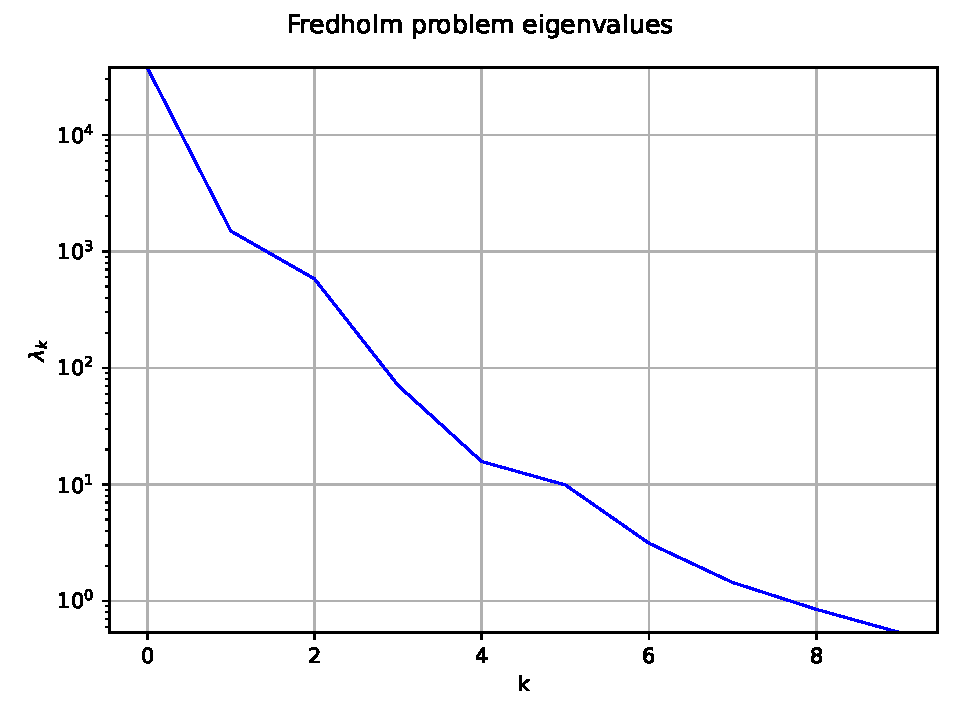
\includegraphics[width=.75\textwidth]{figures/EigenValues.pdf}
    
\column{0.5\textwidth}
        
\tiny
\begin{lstlisting}[language=Python, numbers = none]
meanField = outputField.computeMean()
meanFunction = ot.P1LagrangeEvaluation(
	meanField)
trend = ot.TrendTransform(meanFunction, mesh)
invTrend = trend.getInverse()
outputFieldCentered = invTrend(outputField)

truncThreshold = 1.0e-5
algo = ot.KarhunenLoeveSVDAlgorithm( 
	outputFieldCentered, truncThreshold)
algo.run()
KLResult = algo.getResult()

eigenValues = KLResult.getEigenvalues()
\end{lstlisting}

\end{columns}


\end{frame}


% %%%%%%%%%%%%%%%%%%%%%%%%%%%%%%%%%%%%%%%%%%%%%%%%%%%%%%%%%%%%%%%%%%%%%%%%%%%%%

\begin{frame}[containsverbatim]
\frametitle{Dimension reduction: Karhunen-Loeve decomposition}

\scriptsize 

\begin{equation*}
\tilde{Y}(\omega, \underline{t}) =  \sum_{k=1}^{p} \sqrt{\lambda_k} \xi_k(\omega)\underline{\varphi}_k(\underline{t})
\end{equation*}

Main modes:

\begin{columns}
    \column{0.5\textwidth}

    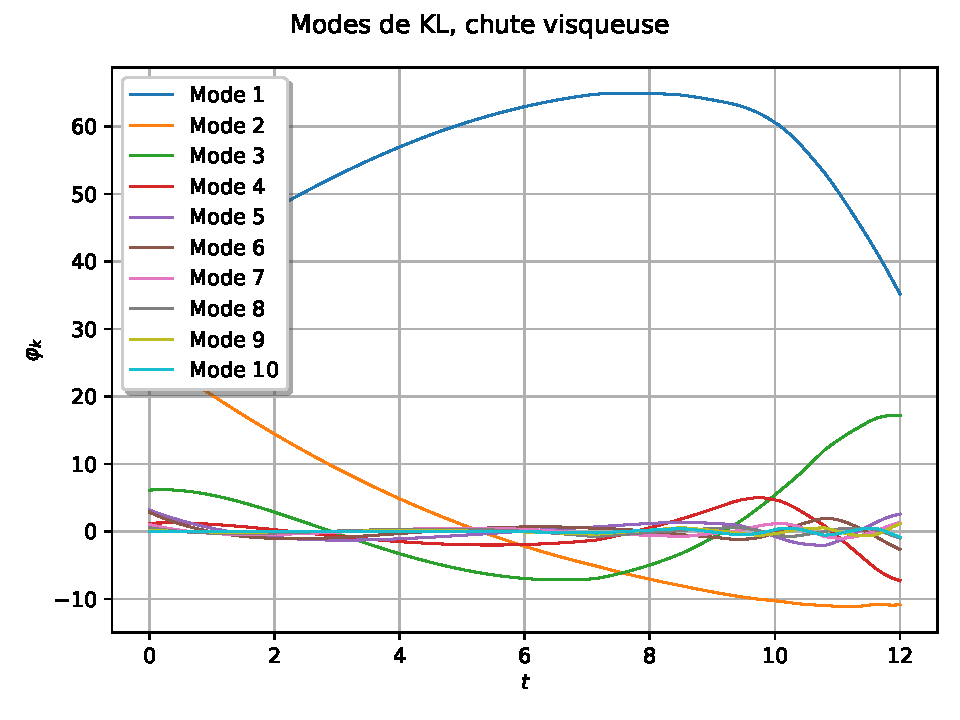
\includegraphics[width=1.\textwidth]{figures/Modes.pdf}
    
\column{0.5\textwidth}
        
\tiny
\begin{lstlisting}[language=Python, numbers = none]
scaledModes =
 KLResult.getScaledModesAsProcessSample()
graph = scaledModes.drawMarginal(0)
graph.setTitle('Modes de KL, chute visqueuse')
graph.setXTitle(r'$t$')
graph.setYTitle(r'$\varphi_k$')
leg = ot.Description([ 'Mode '+str(i +1) for
	 i in range(eigenValues.getDimension()) ])
graph.setLegends(leg)
graph.setLegendPosition('topleft')
view=View(graph)
\end{lstlisting}

\end{columns}


\end{frame}

% %%%%%%%%%%%%%%%%%%%%%%%%%%%%%%%%%%%%%%%%%%%%%%%%%%%%%%%%%%%%%%%%%%%%%%%%%%%%%

\begin{frame}[containsverbatim]
\frametitle{Dimension reduction: Karhunen-Loeve decomposition}

\scriptsize

We only consider the first 2 terms of the decomposition:

\centering
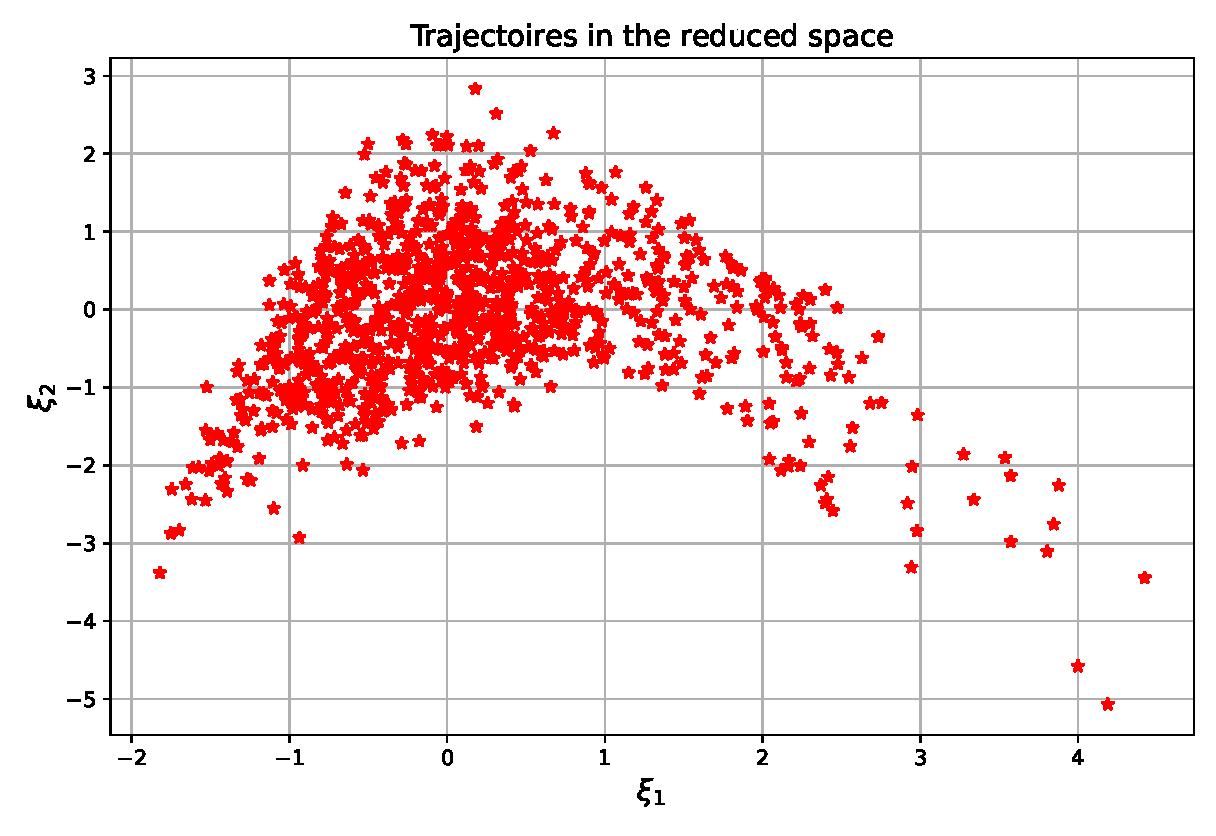
\includegraphics[width=.7\textwidth]{figures/Reduced_Space.pdf}

\begin{lstlisting}[language=Python, numbers = none]
projectionFunction = ot.KarhunenLoeveProjection(KLResult)
sampleKsi = projectionFunction(outputFieldCentered)
sampleKsi = sampleKsi[:,:2]
\end{lstlisting}

\end{frame}

% %%%%%%%%%%%%%%%%%%%%%%%%%%%%%%%%%%%%%%%%%%%%%%%%%%%%%%%%%%%%%%%%%%%%%%%%%%%%%

\begin{frame}[containsverbatim]
\frametitle{Field function analysis}

\scriptsize

We center the trajectories with respect to the mean field:

\begin{minipage}[t]{0.5\textwidth}
    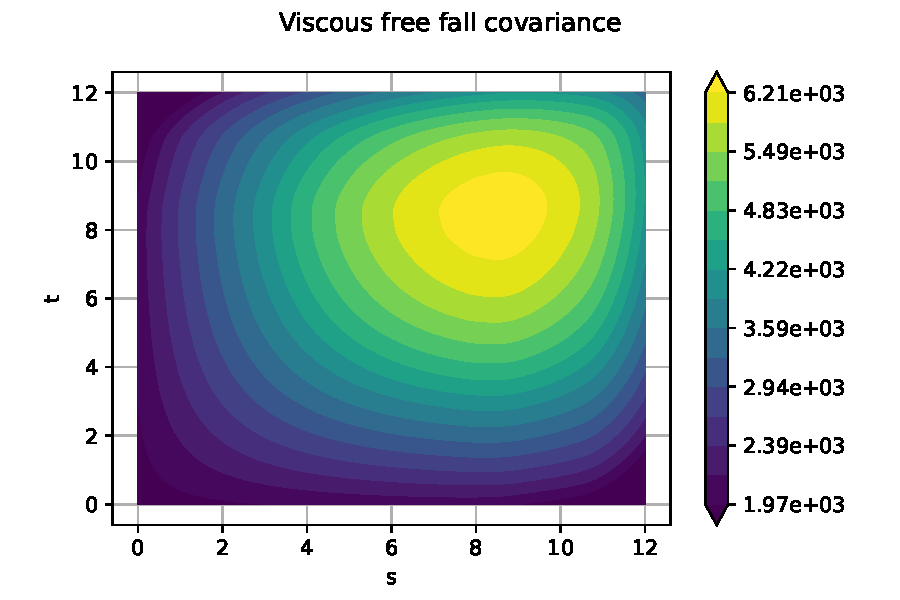
\includegraphics[width=\textwidth]{figures/Covariance.pdf}
\end{minipage}%
\begin{minipage}[t]{0.5\textwidth}
    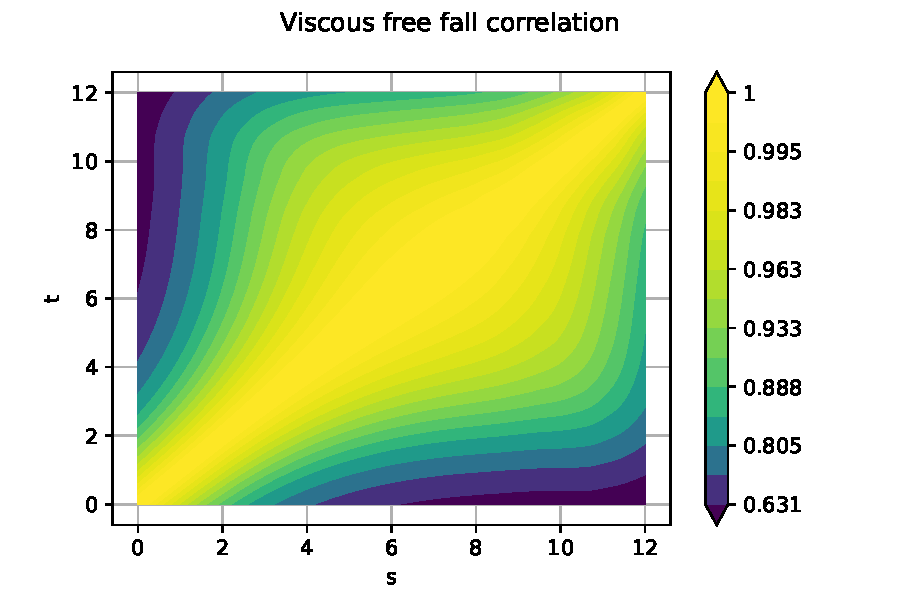
\includegraphics[width=\textwidth]{figures/Correlation.pdf}
\end{minipage}


\begin{lstlisting}[language=Python, numbers = none]
cov = KLResult.getCovarianceModel()

# As a covariance function
isStationary = False
asCorrelation = False
graph = cov.draw(0, 0, tmin, tmax, 128, isStationary, asCorrelation)

# As a correlation function
asCorrelation = True
graph = cov.draw(0, 0, tmin, tmax, 128, isStationary, asCorrelation)
\end{lstlisting}
\end{frame}




%%%%%%%%%%%%%%%%%%%%%%%%%%%%%%%%%%%%%%%%%%%%%%%%%%%%%%%%%%%%%%%%%%%%%%%%%%%%%
%%%%%%%%%%%%%%%%             PERSALYS                        %%%%%%%%%%%%%%%%
%%%%%%%%%%%%%%%%%%%%%%%%%%%%%%%%%%%%%%%%%%%%%%%%%%%%%%%%%%%%%%%%%%%%%%%%%%%%%
%%%%%%%%%%%%%%%%%%%%%%%%%%%%%%%%%%%%%%%%%%%%%%%%%%%%%%%%%%%%%%%%%%%%%%%%%%%%%
\section{Persalys Overview}
%%%%%%%%%%%%%%%%%%%%%%%%%%%%%%%%%%%%%%%%%%%%%%%%%%%%%%%%%%%%%%%%%%%%%%%%%%%%%
\begin{frame}{Project overview}
  \begin{itemize}
  \item
    Partnership between EDF and Phimeca since 2015
  
    \begin{itemize}
    \item
      Developed in C++ using Qt
    \item
      Aiming at maximizing the use of OpenTURNS - through a dedicated GUI
      - for engineers/researchers without a strong coding experience
    \item
      As easy to use as possible while providing the user with help and
      guidelines
    \item
      Benefit from the advanced visualization capability of
      Paraview
    \end{itemize}
  \end{itemize}
  \end{frame}
  
  \begin{frame}{}
  \protect\hypertarget{section}{}
  \begin{itemize}
  
  \item
    Features:
  
    \begin{itemize}
    
    \item
      Uncertainty quantification:
    \item
      Probabilistic model definition
    \item
      Distribution fitting
    \item
      Probability estimate
    \item
      Metamodeling
    \item
      Screening
    \item
      Optimization
    \item
      Design of experiments
    \item
      As generic as possible
  
      
      \item
        Allows for a wide variety of models
      \item
        Can be coupled to external code
    \item
      GUI language in both English and French
    \end{itemize}
  \item
    LGPL license
  \item
    Two releases per year, follows OpenTURNS development
  \item
    Available for free on demand at
    \url{https://persalys.fr}
  
  \end{itemize}
  \end{frame}
  
  \begin{frame}{Persalys installation}
  \protect\hypertarget{persalys-installation}{}
  \begin{itemize}
  
  \item
    Github: sources
  \item
    You can request executables at
    \url{https://persalys.fr/obtenir.php?la=en}
  \item
    Depending on your OS
  
    \begin{itemize}
    
    \item
      \href{https://openturns.github.io/openturns/1.22/usecases/use_case_logistic.html}{Linux} $\rightarrow$ .AppImage (600 Mo)
    \item
      Windows $\rightarrow$ .exe will create a shortcut on your Desktop
      (program is 1.45 Go)
    \end{itemize}
    \item Also distributed by Debian-based GNU/Linux distributions (e.g. Debian, Ubuntu...)
  \end{itemize}
  \end{frame}

  \begin{frame}{Open Persalys and click on ``New study''}
    \centering
    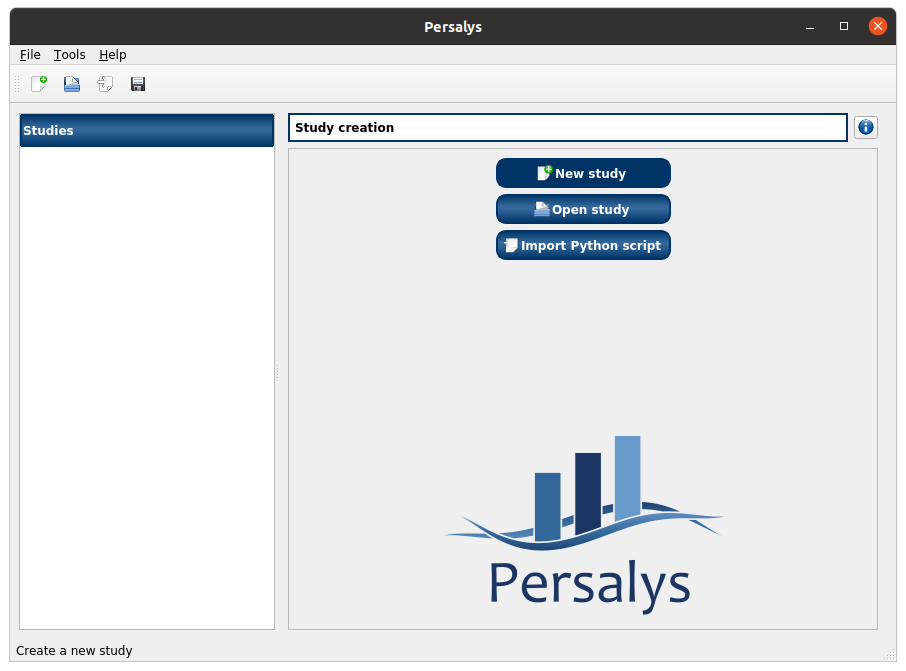
\includegraphics[width=.89\textwidth]{figure/Persalys_GUI.png}
    \end{frame}
    
    \begin{frame}{Create a study}
    
    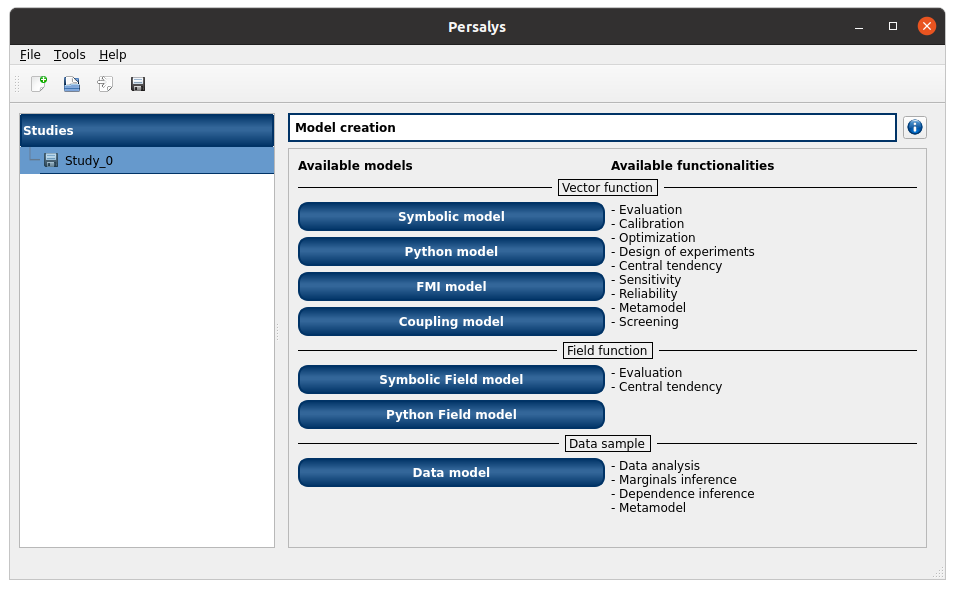
\includegraphics[width=\textwidth]{figure/Persalys_new_study.png}
    \end{frame}
    
    \begin{frame}{Definition/Evaluation}
    \protect\hypertarget{definitionevaluation}{}
    Models are viewed as a ``black box'' with inputs, outputs and a
    transfer function (TF).
    Persalys supports two model categories:
    
    \begin{itemize}
    \item
      vector to vector (\(X_i \rightarrow Y_i\), emphasized here)
    \item
      vector to 1D field (\(X_i \rightarrow Y_i(t)\))
    \end{itemize}
    
    \medskip

    Vector to vector models can be of the following type:
    
    \begin{itemize}
    
    \item
      Symbolic, TF is a mathematical formula
    \item
      Python, TF is a Python function
    \item
      FMI, TF is provided by an FMU model
    \item
      Coupling, TF is an executable command which reads/writes input/output
      files
    \end{itemize}
    \end{frame}
    
    \begin{frame}{Coupling model definition}
    
    \centering
    
    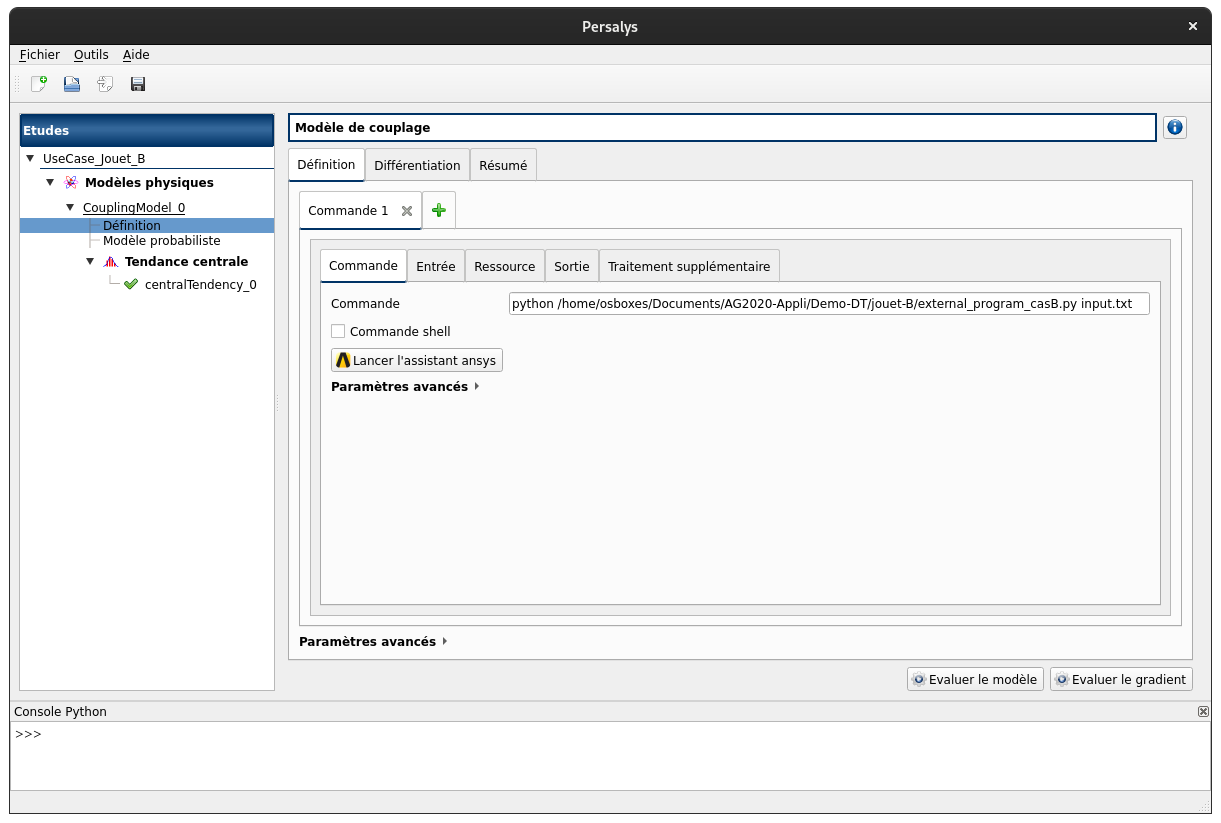
\includegraphics[width=0.97\textwidth]{figure/model_definition.png}
    
    \end{frame}
    
    \begin{frame}{Study workflow}
      \centering
      
      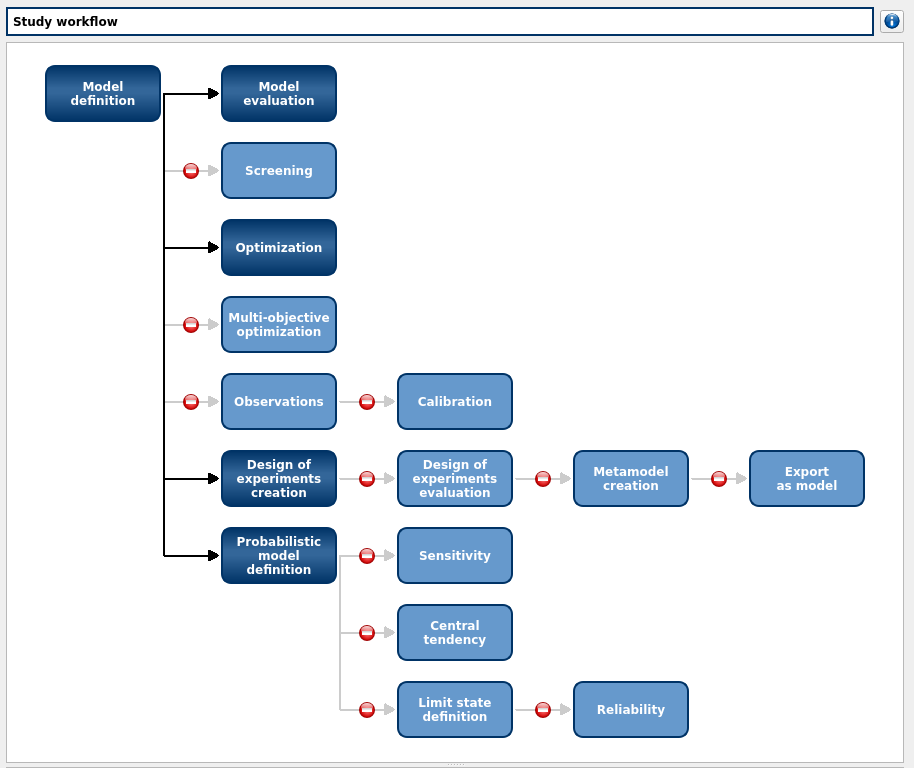
\includegraphics[width=0.7\textwidth]{figure/StudyWorkflow.png}
      
      \small
      Blocks become available as study content grows and prerequisites are fulfilled.
      \end{frame}

\begin{frame}{Probabilistic models}
  \small
  Each input variable can be associated to a distribution.
  
  Dependencies
  between variables are specified as copulas.
  
  \centering
  
  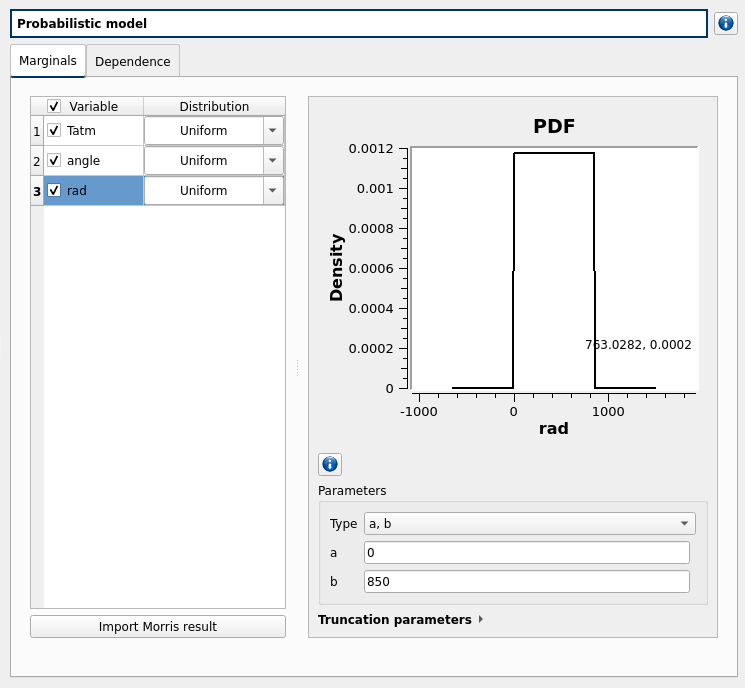
\includegraphics[width=0.63\textwidth]{figure/overviewProbaModel.png}
  
  \end{frame}

  \begin{frame}{Metamodel (surrogate model) creation}
    \small
    Using an evaluated design of experiments, the user can build a surrogate model (linear
    regression, functional chaos or Gaussian process regression). Validation
    tests are run to check the approximation being made.
    
    \centering
    
    \includegraphics[width=0.59\textwidth]{figure/overviewMetamodel.png}
    
    \end{frame}
%%%%%%%%%%%%%%%%%%%%%%%%%%%%%%%%%%%%%%%%%%%%%%%%%%%%%%%%%%%%%%%%%%%%%%%%%%%%%




\begin{frame}

\begin{block}{OpenTURNS resources}
\begin{itemize}
    \item Website and documentation: \url{www.openturns.org}
    \item GitHub: \url{https://github.com/openturns/openturns}
    \item Forum: \url{https://openturns.discourse.group}
\end{itemize}    
\end{block}

\begin{block}{Persalys resources}
\begin{itemize}
    \item Website and documentation: \url{https://persalys.fr/?la=en}
    \item Forum: \url{https://persalys.discourse.group}
\end{itemize}    
\end{block}

\begin{columns}
\column{0.5\textwidth}
\centering
\includegraphics[width=0.5\textwidth]{figures/logo-openturns.png}
\column{0.5\textwidth}

\includegraphics[width=0.8\textwidth]{figures/PERSALYS-LOGO.png}

\end{columns}

\end{frame}
  
\end{document}